\chapter{Role of geometry, charge and fluxionality of clusters in CO\texorpdfstring{$_2$}{} activation on supported sub-nanometer metal clusters: the case of Cu tetramers on pristine and O-terminated MXene}\label{appendix2}
\footnotetext[1]{Reprinted (adapted) with permission from \texorpdfstring{\emph{Catalysis Today}}{}, \texorpdfstring{\textbf{2021}}{}, 370, 93-103}


%%%%%%%%%%%%%%%%%%%%%%%%%%%%%%%%%%%%%%%%%%%%%%
Reduction of CO$_2$ to useful chemicals using supported few atom copper clusters has been an active area of research. The first step in this process is chemisorption and reduction of CO$_2$ to CO$_2^{\delta-}$. Previous studies have shown that the ease of chemisorption depends on the cluster geometry and charge. In an effort to elucidate the role of cluster-support interactions and thereby cluster geometry, charge on cluster on CO$_2$ chemisorption, in this work, using density functional theory based calculations, we have studied the physisorption and chemisorbtion of CO$_2$ on Cu tetramers supported on pristine and O-terminated Ti$_2$C MXene. Our calculations show that for CO$_2$ to exhibit exothermic adsorption, the cluster should (a) wet the support thereby exposing all the Cu atoms to the  approaching CO$_2$ molecule, (b) be preferably positively charged with Cu atoms present in more than one oxidation state and (c) be fluxional on the support. Our nudged elastic band based calculations show that the transition from physisorbed to chemisorbed CO$_2$ is an activated process. Amongst the systems considered in this study, the activation barrier is usually low except on the tetrahedral cluster on the oxygen terminated Ti$_2$C support.



\section{Introduction}

 Carbon dioxide (CO$_2$), primarily produced from combustion of fossil fuels and natural
 gas, is one of the primary agents for air pollution, ocean acidification\cite{cc} and
 adverse global climate changes\cite{climate}. A green way to diminish this problem is
 to capture CO$_2$ from atmosphere and convert it to inexpensive and easily available
 feedstock to produce chemicals and fuels like short-chain olefins, syngas, formic acid,
 methanol, etc\cite{dorner, javier}. The most alluring way to do this conversion is the 
 hydrogenation of CO$_2$ to methanol\cite{hydrogenation1, hydrogenation2} or reduction to 
 carbon monoxide (CO) through reverse water gas shift (rWGS) reaction\cite{rwgs}. While methanol is used as an alternative
 fuel, the later can
 be used as a starting material for other industrially important reactions. Hence CO$_2$ capture,
 utilization and storage using heterogeneous and homogeneous catalyst has been a major
 area of research.
 
 However, one of the main challenges in achieving the above is the unusually high stability of
 CO$_2$ that results in elevated barriers for chemical reactions on many catalysts. The
 difficulty is further aggravated by the fact that there is a need for high enough
 adsorption energy for the catalyst to retain the adsorbate. On the positive side CO$_2$
 posses a significant amount of quadrapole moment that enables strong interaction between
 CO$_2$ and the specific binding sites in the catalyst\cite{kunkel}. Therefore, in presence of 
 a suitable catalyst, the barriers can be significantly reduced. 
 
 Industrial catalysts typically use metal nanoparticles dispersed on an oxide
 support. For eg. commercial catalysts for conversion of CO$_2$ to methanol are typically Cu based, 
 containing ZnO and/or Al$_2$O$_3$\cite{com1,com2}. While at low
 temperatures they show poor activity, at high temperatures the rWGS is favoured resulting is low yield of methanol.
 Further, formation of water facilitates sintering of Cu and ZnO, thereby deactivating the
 catalyst. Therefore, there are efforts to design novel catalysts for conversion of CO$_2$
 to methanol at low temperatures.
 
 Fundamental investigations of CO$_2$ conversion on extended Cu surfaces like the low
 indexed (111), (100) and (110) indicate that CO$_2$ interacts weakly with the surfaces, thereby
 resulting in low yield \cite{lang2012gas, yang2010fundamental, campbell1989sr, schneider1992interaction, grabow2011mechanism, zhang2018optimum}.
 In contrast, one observes enhanced
 reactivity when Cu or Au nanoparticles are dispersed on transition metal oxide or carbide
 supports and vice-versa \cite{rodriguez2015hydrogenation, zhang2018optimum}
 Further, Yang \textit{et al.}
 showed that the yield of converted methanol is enhanced when Au nanoparticles are activated on a
 CeO$_x$/TiO$_2$ interface\cite{rodriguez2015hydrogenation}.
 On transition metal carbides, it was shown that Au$_4$ and Cu$_4$ clusters are highly reactive
 with a strong binding of CO$_2$. Density functional theory (DFT) based calculations showed that
 the cause for such high reactivity can be attributed to the charge polarization induced due to cluster-support interactions\cite{vidal2012co2, rodriguez2007adsorption, gomez2011reactivity}.
 However, it was observed that as the cluster size is
 increased the electron redistribution was attenuated that resulted in significantly reduced
 reactivity\cite{vidal2012co2, rodriguez2007adsorption, gomez2011reactivity}.
 These studies suggest that small metal clusters on oxide/carbide supports are good candidates
 for CO$_2$ capture and utilization. In addition to their size, the reactivity of clusters of a given size also depends on the support as shown in the studies of CO$_2$ conversion to methanol on
 Cu/TiO$_2$(110)\cite{graciani2014highly}
 and Cu/Zn(000$\bar{1}$ surfaces \cite{yang2017copper}.


 Irrespective of the final product, the primary condition any catalyst needs to satisfy is that
 CO$_2$ should be chemisorbed, such that it is activated. Moreover, as observed in previous
 studies, in the chemisorbed state, an electron is transferred from the catalyst to CO$_2$, 
 resulting in an activated anionic CO$_2^{\delta -}$ species\cite{mxene-co2, freund}. The ease with which
 this charge transfer occurs depends on the relative position of the frontier orbitals (both occupied
 and empty) of the cluster and the CO$_2$ molecule. For the cluster this is controlled by the interaction
 with the support. Previous studies show a lot of variations in the cluster shape and charge depending on the type
 of support. This in turn results in significant changes in the
 geometry and strength of CO$_2$ adsorption. For example, it was
 shown that Cu$_4$ on TiO$_2$(110) surface has a tetrahedral geometry\cite{tao2019best}.
  The Cu atoms interacting with TiO$_2$ are positively charged while that on the vertex remains more or less
 neutral. On this cluster CO$_2$ binds at the metal-oxide interface, rather than binding
 on the cluster itself, with a binding energy of about -0.85 eV. In contrast, on transition metal-carbides Cu$_4$ forms a rhombus wetting the surface. However, the charge on the cluster and the
 CO$_2$ adsorption energies differ depending on the transition metal present in the carbide and the surface
 termination. DFT based studies of CO$_2$ adsorption
 on Cu$_4$ supported on TiC(001) surface show that the cluster is negatively charged. CO$_2$ binds to the cluster
 with a binding energy of -1.12 eV \cite{vidal2012co2}.
 Upon changing the substrate to 
 $\delta$-MoC(001), it was found that both the tetrahedral and rhombus geometries are almost isoenergetic, with the
 rhombus lying horizontally on the surface to be slightly lower in energy. Though on TiC and $\delta$-MoC the geometries are same, the charge and CO$_2$ binding energies are significantly different. In contrast with the TiC(001) surface, on $\delta$-MoC(001) it was shown that  the cluster was positively charged and CO$_2$ binds with a binding energy of -0.60 eV\cite{posada2016highly}.

 
 Inspite of the variations pointed above, we note that, to the best of our knowledge, there is no
 systematic study to understand correlations between the support properties, the charge on the cluster
 and the nature of CO$_2$ adsorption and activation on them. For example, is it better to have clusters
 that wet the surface or have a three-dimensional structure? Does CO$_2$ prefer to adsorb preferentially on
 a cluster depending on its charge? Further, it would also be interesting to study whether there
 is any barrier involved for converting CO$_2$ from its physisorbed state to chemisorbed state. We note that on
 some low-indexed transition metal carbide surfaces, Quesne  \textit{et al.} found that the transition from physisorption to chemisorption involves a barrier \cite{quesne2019carbon}.
  With these questions in mind we have studied CO$_2$ adsorption and activation on Cu$_4$ clusters supported on Ti$_2$C-MXene, both pristine and O-terminated. We have chosen Cu$_4$ because it is not only well studied (as described in the previous paragraphs) but also is the most efficient one\cite{tao2019best}.
 Ti$_2$C MXene is chosen as the support because of the following reasons. It is a form of carbide with a relatively
 simple structure; the surface has only Ti atoms present. Also its work function can be tuned easily by considering
 O-terminated Ti$_2$C MXene (Ti$_2$CO$_2$). Additionally, MXenes with tunable surface terminations have diverse 
 properties ranging from energy storage\cite{anasori20172d} to catalysis\cite{li20192d, zhang2017ti, li2015heterogeneous}. In the domain of catalysis, O-terminated  Ti$_2$C MXene have shown to have huge potential as electrocatalysts for hydrogen evolution reaction\cite{gao20162d} and CO$_{2}$ reduction reaction\cite{li2015heterogeneous}. In contrast, to the best of our knowledge, their role as a support to TM clusters have not been explored.
 
 The rest of the chapter is arranged as follows: In Section \ref{compdett} we describe the details of the
 computational methods used in this study. The results, that include properties of the gas phase clusters,
 clean supports, clusters adsorbed on the supports and CO$_2$ adsorbed on the supported clusters, are presented
 in Section \ref{resultsss}. In this section we also describe the role of cluster charge and geometry on the adsorption
 process and the barriers involved from going to a physisorbed to a chemisorbed configuration. The results
 are summarized in Section \ref{concll}.


\section{Computational details }
   \label{compdett}
Spin-polarized DFT based calculations were performed using the Quantum ESPRESSO (QE) 
software\cite{QE2009}. The electron exchange and correlation were approximated within the 
generalized gradient (GGA) framework proposed by Perdew, Burke and Ernzerhof 
(PBE)\cite{GGA-PBE1996}. Ultrasoft pseudopotentials\cite{USPP1990} were used to describe the 
electron-ion interactions. The pseudopotentials used for the different elements have the following 
valence configurations: (a) Ti : [3$s{^2}$,3$p{^6}$,3$d{^2}$,4$s{^2}$] , (b) Cu : 
[3$d^{10}$,4$s{^1}$], (c) O : [2$s{^2}$,2$p{^4}$], (d) C : [2$s{^2}$,2$p{^2}$], and (e) H : 
[1$s^1$]. The wave functions and charge density were expanded in a plane wave basis with kinetic 
energy cutoffs of 55 Ry and 480 Ry respectively. 
 
For the clean Ti$_2$C and Ti$_2$CO$_2$ substrates, the Brillouin zone (BZ) integrations for a (1 
$\times$ 1) surface unit cell were carried out with a 12 $\times$ 12 $\times$ 1 shifted 
Monkhorst-Pack k-point mesh \cite{K-pointMP1976}, while for the clusters in the gas phase BZ 
integrations are done using the $\Gamma$-point only. Marzari-Vanderbilt smearing 
\cite{SmearingMV1999} with a smearing width of 0.007 Ry was used to expedite the convergence of electronic 
energy. 

Since for the clusters in the gas phase (the support and 
the supported clusters), the artificial periodicity along all 
the three directions (directions perpendicular to the plane of the support) introduces spurious interactions with the
periodic images, we have considered a large enough vacuum along the directions of artificial periodicity to minimize these spurious interactions. The gas phase clusters were kept in a large cubic box such that there is a minimum distance of about  10 {\AA} between periodic images in all directions. For the substrates with and without the clusters, we have used a vacuum thickness of at least 12 {\AA} along the direction normal to the substrate. Further, in this study, we are interested in interactions between the clusters and
the support. Hence for the clusters on the support, we have used supercells of Ti$_2$C and Ti$_2$CO$_2$ to avoid interaction along the x-y direction amongst the periodic images of the clusters. To model the supported clusters, we have used a (4 $\times$ 4) supercell of the support. This supercell ensure a minimum of 9 {\AA} separation between the periodic images of the clusters along the xy plane. Moreover, in accordance with the supercell we have used a 3$\times$3$\times$1 k-point mesh for BZ integrations. 



The thermodynamic stability of the clusters in the gas phase is studied by computing the binding energy ($E_{bind}$),
which is given by:
\begin{equation}
 E_{bind} = [E^{g}_{Cu{_n}}-{nE^{g}_{Cu{_1}}}]/n
 \label{Ebind}
\end{equation}
where, $n$ is the number of atoms in the cluster and $E^{g}_{Cu_n}$ is the total energy of the 
Cu$_n$ cluster in the gas phase. A negative value of $E_{bind}$ indicates that the clusters are stable compared to that of the isolated atoms.

In order to determine the structure of O-terminated Ti$_2$C MXene we computed the O binding energy ($E^O_{b}$) on 
Ti$_2$C, which is given by:
\begin{equation}
 E^O_{b} = [E_{Ti_2CO_2} - E_{Ti_2C} - E^{g}_{O_2}]/2 
 \label{ebindO}
\end{equation}
where, $E_{Ti_2CO_2}$, $E_{Ti_2C}$ and $E_{O_2}$ are the total energies of Ti$_2$CO$_2$, Ti$_2$C and oxygen molecule respectively.

The formation energy of a 
cluster on support, $E_{form}^S$, provides information about the energy gained when $n$ adatoms
on the support combine to form a cluster of $n$ atoms. This tells us
the stability of the cluster against dissociation to adatoms on the surface and is given by:

\begin{equation}
 E_{form}^S = [E_{Cu{_n}/X} - n*E_{Cu{_1}/X} + (n-1)* E_{X}]/n
 \label{Ef}
\end{equation}

The overall energetics of the interaction between a cluster and the support or the CO$_2$ molecule
and the supported cluster is given by the adsorption energy ($E_{ads}$). When two species A and B
interacts to form A+B, $E_{ads}$ is given by:

\begin{equation}
 E_{ads} = E_{A+B} - E_{A} - E_{B}
 \label{eads}
\end{equation}
\noindent where $E_{A+B}$, $E_A$ and $E_B$ are the total energies of A+B, A and B respectively.
$E_{ads}$ depends on two competing energy factors, namely, the energy gained due to the interaction between
A and B ($E_{int}$) and the energy cost due to the deformation of A and B because of the interaction.
$E_{int}$ is given by
\begin{equation}
    E_{int}=E_{A+B} - E^{A+B}_A - E^{A+B}_B
     \label{eint}
\end{equation}
\noindent where the second and third terms in the above equation are the total energies of
A and B respectively when they are in the same geometry as that of the interacting
system A+B. The deformation energies are computed as follows:
\begin{equation}
 E^{i}_{def} = E^{A+B}_{i} - E_i
 \label{Edef-s}
\end{equation}

\noindent where $i$ can be either A or B. In our study, A and B can be the Cu$_4$ and the support
respectively or they can be CO$_2$ and Cu$_4$+support.

The charge transfer between the adsorbate and adsorbent is quantified by using the Bader charge analysis and is computed as follows:
  \begin{equation}
     \Delta {q} =  q_{A+B} - q_{A} - q_{B}
   \label{charge}
  \end{equation}
where, $q$ denotes the bader charge and $A$ and $B$ denotes the adsorbate and adsorbent
respectively.

The determination of the minimum energy paths and the activation energy for CO$_2$ to be converted from physisorbed to chemisorbed state has been
computed using the climbing-image nudged elastic band (CI-NEB). Depending on the length of the path
we have used a maximum (minimum) of 17 (8) images.

\section{Results and Discussions}
\label{resultsss}
  \subsection{Structure and electronic properties of substrates and Cu\texorpdfstring{$_4$}{} cluster in gas phase}
  
  \noindent \textit{Pristine Ti$_{2}$C MXene:} 
  Ti$_2$C MXene forms a two-dimensional hexagonal lattice with a layer of C atoms sandwiched between two layers of Ti atoms (Figure~\ref{fig:1}(a))\cite{khazaei2013novel}\cite{naguib2012two}. The three layers of Ti-C-Ti have an ABC stacking. Each carbon atom is bonded to six Ti atoms in an octahedral geometry, while each Ti atom in either layer is bonded to three C atoms. We obtain a lattice parameter of 3.06 {\AA} that is in excellent agreement with previous calculations\cite{gan2013first}\cite{gao2016monolayer}. An unpaired electron on Ti atom makes the system magnetic. Spin polarised calculations reveal that
  in its most stable configuration, the intralayer (interlayer) magnetic coupling between Ti atoms is ferromagnetic (antiferromagnetic) with a magnetic moment of 0.93 $\mu_B$/Ti atom. The   density of states plot in Figure~\ref{fig:1}(b) shows that there is a small band gap of   about 0.29 eV. Both the conduction and valence band edges are primarily from Ti-$3d$ states.

\begin{figure}[ht]
 \begin{center}
    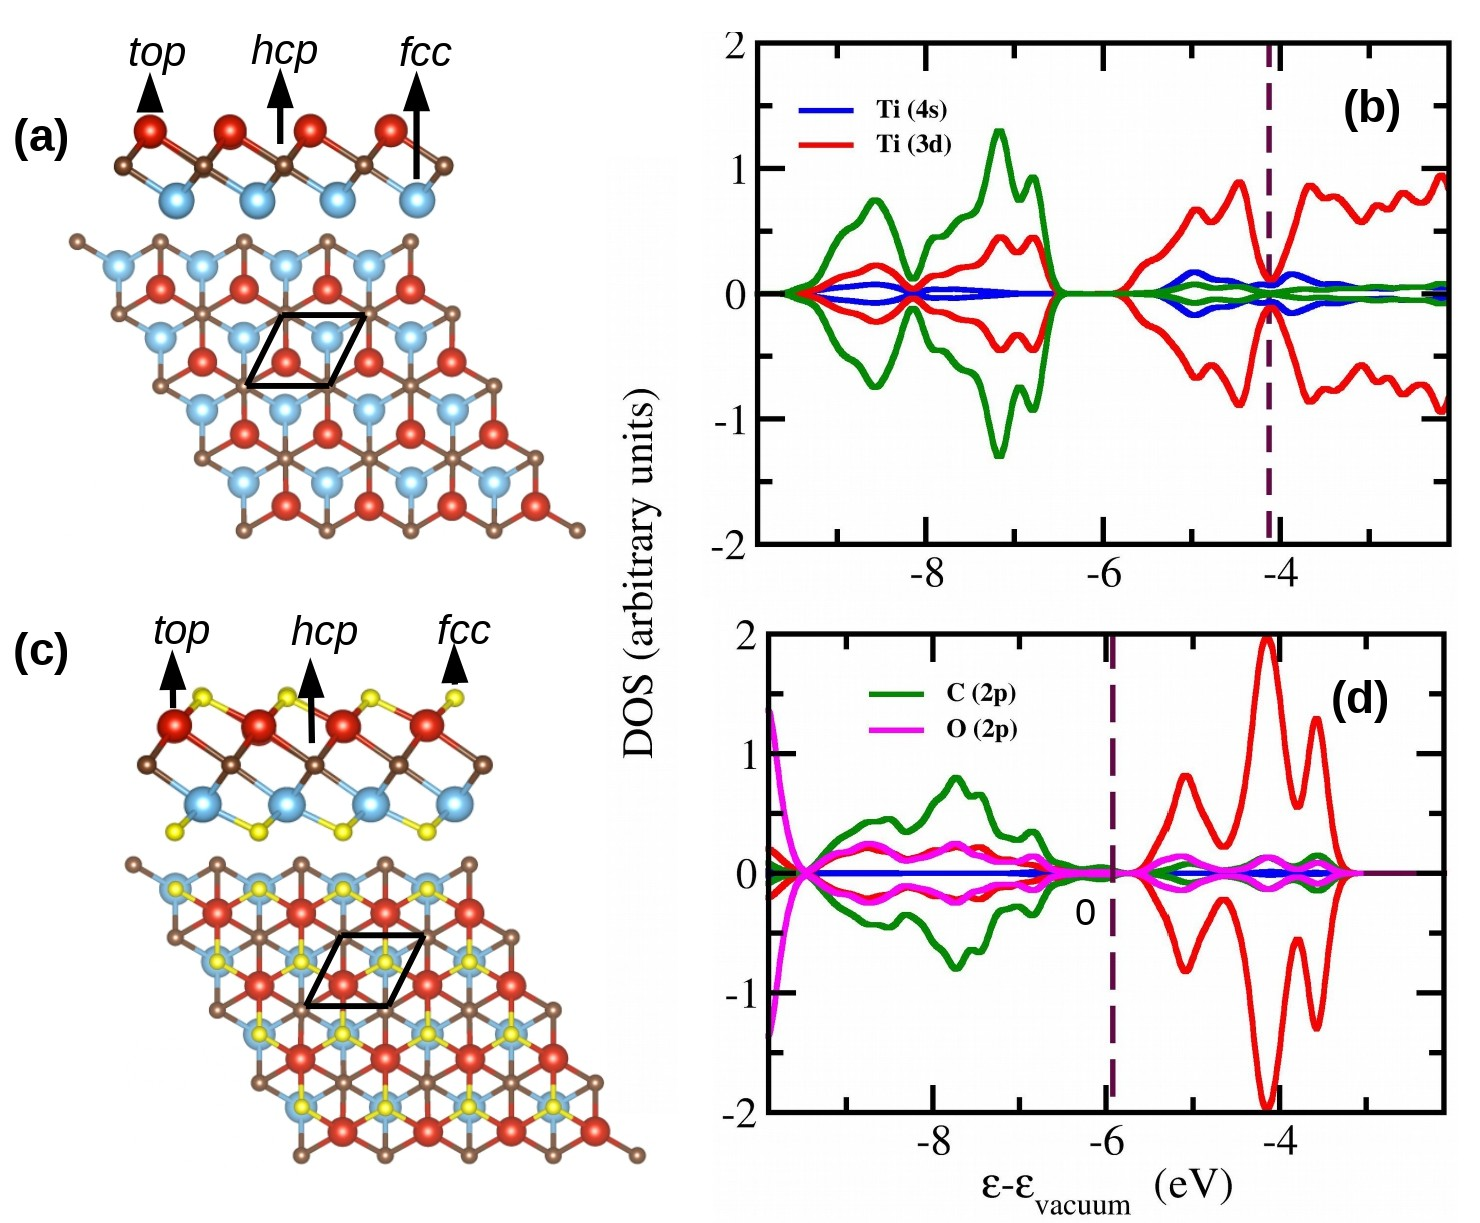
\includegraphics[width=12cm]{Appendix2/Appendix2_figures/mxene.jpg} \\[0cm]
 \end{center}
 \caption{Side and top views of (a) Ti$_2$C MXene and (c) O-terminated Ti$_2$CO$_2$ MXene along with the three adsorption sites ({\it fcc},{\it hcp} and {\it top}). In this and the following figures red, light blue, brown and yellow spheres represent top Ti, bottom Ti, C and O atoms
 respectively, belonging to 
 Ti$_2$C and Ti$_2$CO$_2$ . (b) and (d) shows the DOS projected on $s$ and $d$ states of Ti
 and $p$ states of C and O atoms in Ti$_2$C and Ti$_2$CO$_2$ respectively.}
  \label{fig:1}
\end{figure}


 \noindent \textit{O-terminated Ti$_2$C MXene (Ti$_2$CO$_2$)}: On Ti$_2$C surface O can 
 adsorb either on {\it top} of a Ti atom or on one of the two 3-fold hollow sites,  namely {\it fcc} and {\it hcp} (Figure~\ref{fig:1}(a)). In the {\it fcc}-site the  adsorbate will be above the Ti atom in the bottom layer, while in case of {\it hcp} it 
 will be above the C atom. Considering the fact that both the top and the bottom  surfaces have O adsorbed on them, six different configurations of Ti$_2$CO$_2$ were  considered (Figure S1 in SI). The most stable configuration is the one where 
 O is adsorbed at the {\it fcc} site on both the surfaces (Figure \ref{fig:1}(c)). The 
 lattice parameter (3.03 {\AA}) and formation energy (-5.06 eV/atom) of Ti$_2$CO$_2$ are
 in excellent agreement with existing literature\cite{khazaei2013novel}. Our 
 calculations show that Ti$_2$CO$_2$ is a semiconductor with a band gap of 0.34 eV, 
 which agrees well with previous PBE-based calculations.\cite{khazaei2013novel} 


In contrast to Ti$_2$C, where states near the band edges are primarily from Ti-$d$ orbitals (Figure \ref{fig:1}(b)), for Ti$_2$CO$_2$, the valence and conduction
bands results from hybridization of the Ti-$d$ and C and O-$p$ states. The
valence band edge has largest contribution from C-$p$. It also has significant contribution from O-$p$ states (Figure \ref{fig:1}(d)). The conduction band
edge states arise primarily from Ti-$d$. The presence of more electronegative O above 
Ti results in transfer of charge from the Ti atoms to the O atoms. As a consequence of this, we find that the work function of Ti$_2$CO$_2$ increases to 5.92 eV from that of 4.13 eV in the case of Ti$_2$C.


\noindent \textit{Copper tetramer (Cu$_4$) in gas phase:} Neutral copper clusters in gas phase have been well studied theoretically \cite{guvelioglu2006first, guvelioglu2005evolution, chaves2014role, calaminici1996density}. Based on previous studies, we have considered two configurations for the tetramer in the gas phase, namely the rhombus (cluster has a two-dimensional (2D) structure) and the tetrahedron 
(cluster has a three-dimensional (3D) structure). The optimized geometries of both the 
clusters are shown in Figure~\ref{fig:2}(a) and (c).
In agreement with literature report\cite{guvelioglu2006first} we find that the rhombus is about 0.92 eV lower in energy than the tetrahedron. In the rhombus geometry the Cu atoms have a binding energy of -1.47 eV/Cu atom. Compared to bulk Cu, where the cohesive energy is -3.32 eV/Cu atom, for the rhombus Cu$_4$, the binding energy is almost half. The Cu-Cu bond lengths are of 2.41 \AA. 
Moreover, the distance between two Cu atoms along the long diagonal of the rhombus is about 4.25 \AA, while that between the short diagonal is about 2.30 \AA. The Cu-Cu bond lengths of the tetramer in its 3D tetrahedral configuration is about 2.42 \AA.


Figure~\ref{fig:2}(b) and (d) show the density of states plot of the rhombus
and tetrahedral tetramer. While the rhombus is non-magnetic, we find that the tetrahedral
configuration of the cluster has a magnetic moment of  2 $\mu_B$. In accordance with their relative stability, we find that the highest occupied molecular orbital (HOMO) of the rhombus is about 0.51 eV lower in energy than that of the tetrahedron. For both the clusters we observe that the frontier orbitals have dominant contribution from the Cu-$s$ states.


\begin{figure}[ht]
 \begin{center}
    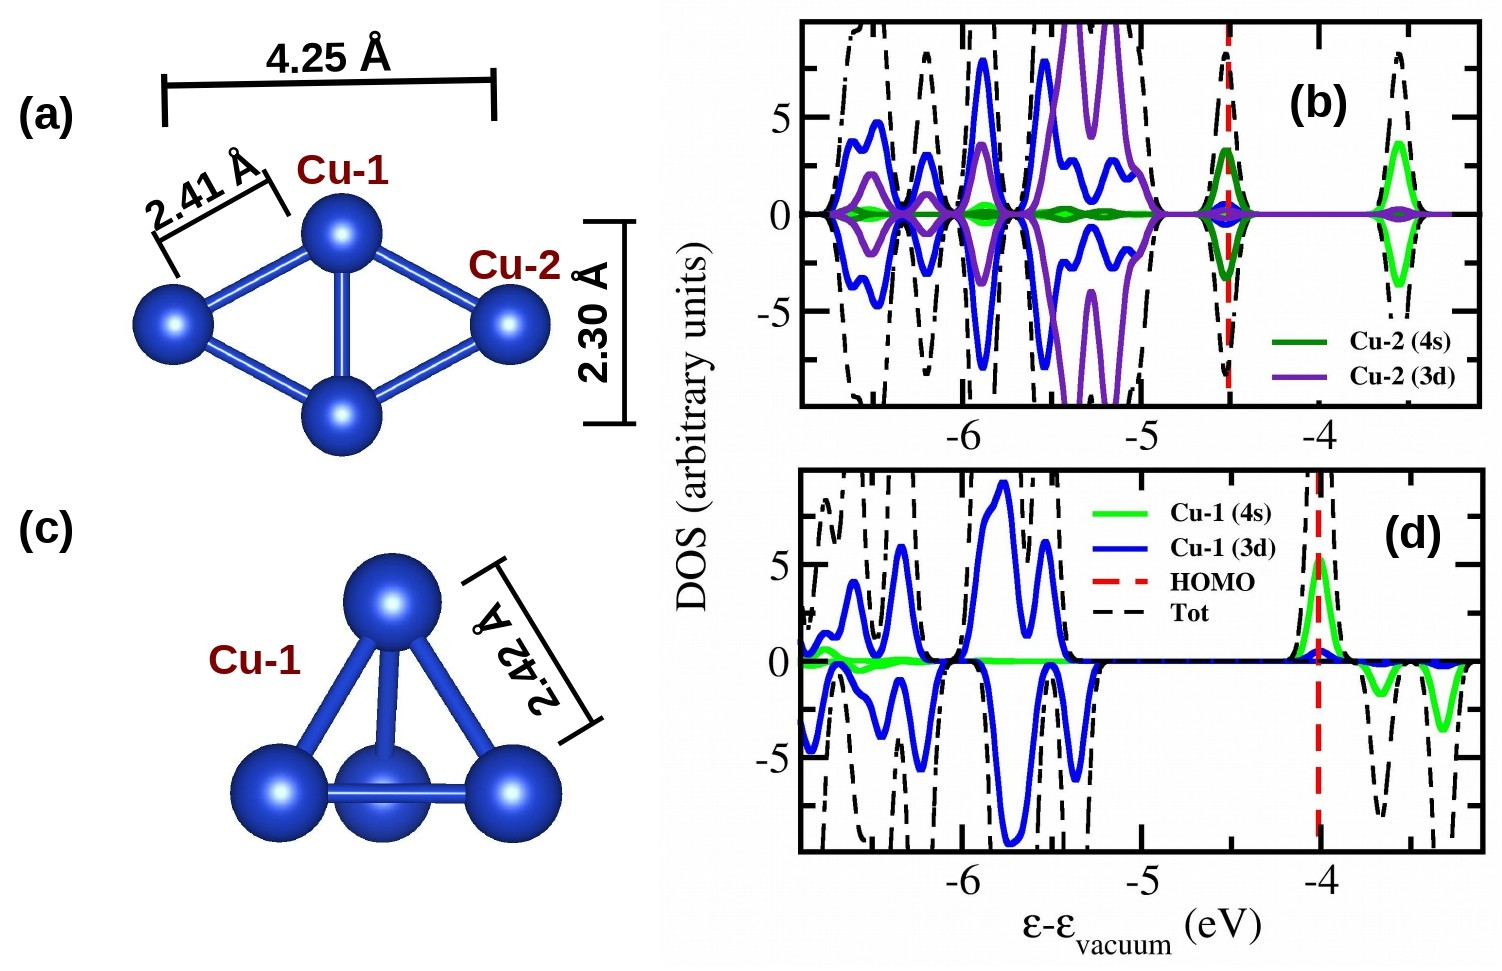
\includegraphics[width=12cm]{./Appendix2/Appendix2_figures/gas_phase_4.jpg} \\[0cm]
 \end{center}
 \caption{ Structure of gas phase copper tetramer cluster (Cu$_4$) in  (a) rhombus  and (c) tetrahedral geometry. In this and the subsequent figures in the chapter, the
 dark blue spheres represents Cu atoms. (b) and (d) show the total DOS and the DOS
 projected on Cu-$d$ and $s$ states for Cu in the rhombus and tetrahedral Cu$_4$ respectively.}
  \label{fig:2}
\end{figure}

\subsection{Copper cluster on support}

\noindent \textit{Cu$_4$ on Ti$_2$C:} On Ti$_2$C surface, the Ti atoms that will be interacting with the
cluster form two types of hollow sites: (a) the fcc site, where the Cu atoms will be above the Ti atoms of the bottom layer and (b) hcp site, where there is C atoms of the second layer will be below the Cu atoms. To determine the lowest energy adsorption configuration of the tetramer on this surface, we have considered six configurations: (i) the tetramer wetting the surface, with the Cu atoms occupying the (a) fcc sites, (b) hcp sites, (c) top sites and (ii) the tetrahedron with three of the Cu atoms interacting with the surface and each occupies either the fcc or the hcp or the top sites, the third Cu atom is adsorbed at the hollow site formed by these three Cu atoms. Moreover, we also considered another configuration in which the tetramer lies
vertically on the surface. The optimized structures for all the cases are shown in Figure S4 of the SI. For both the 2D and 3D configurations we find that the clusters prefer to bind to the fcc hollow site. Similar to the gas phase, we find that the tetramer on the surface prefers a 2D rhombus configuration, thereby wetting the surface, over a 3D tetrahedral one. The rhombus has an adsorption energy of -1.89 eV/Cu atom while the tetrahedron has an adsorption energy of -1.62 eV/Cu atom.

Figure~\ref{cu_ti2c}(a) and (c) show the side and top views of the
lowest energy configurations of the
rhombus and the tetrahedron on Ti$_2$C respectively.
Compared to that observed in the gas phase, for the supported rhombus, the Cu-Cu bond
lengths are significantly elongated to 2.70 \AA. Similarly, the short diagonal of the
rhombus on the surface is also lengthened to 2.63 \AA. In the tetrahedra, we observe that the Cu-Cu bond lengths between the Cu atoms that are interacting
with the surface is also elongated to 2.64 \AA. However, in this case the elongation is about 0.06 \AA~smaller than that observed in the rhombus. In contrast, the Cu-Cu bond lengths between the Cu atoms on the vertex and those at the base is 2.43 \AA, and are similar to that observed in the gas phase.

In order to understand the reason behind the tetramer's preference to wet the surface,
we begin by noting that the preferred adsorption configuration of the cluster on the surface depends on the strength of the Cu-Ti and Cu-Cu interaction. A measure of the strength of these two interactions are given by adsorption energy of Cu adatom  on the surface ($E_{ads}^1$) and the binding energy of the clusters in the gas phase. The former provides a measure of the amount of energy gained by the Ti$_2$C/Cu$_n$ for each Ti-Cu bond formed. However, in order to form Ti-Cu bonds, the Cu-Cu bonds are stretched resulting in an energy cost. The binding energy of the Cu clusters in the gas phase gives a measure of the energy cost associated with the elongation of the Cu-Cu bond. From our calculations we find that a Cu monomer binds strongly to the surface with $E_{ads}^1$=-3.15 eV. This energy is  significantly larger than the binding energy of Cu$_4$ in gas phase (-1.47 eV/Cu atom for rhombus and -1.24 eV/Cu atom for the tetrahedron). Hence the energy gained due to formation of Cu-Ti bonds is significantly larger than the energy cost of stretching the Cu-Cu bonds. Thus, the cluster stabilizes itself by maximizing its interaction with 
the surface, i.e. through formation of more number of Ti-C bonds and in turn wetting the surface.
Further, to estimate the stability of the clusters against dissociation to monomers on the surface, we computed $E_{form}^S$. For the rhombus (tetrahedron), we find that $E_{form}^S$ is -0.20 (+0.06) eV/Cu atom.
This indicates that while the rhombus is stable towards disintegration on the surface, the tetrahedron
might disintegrate to monomers on the support.

\begin{figure}[ht]
 \begin{center}
    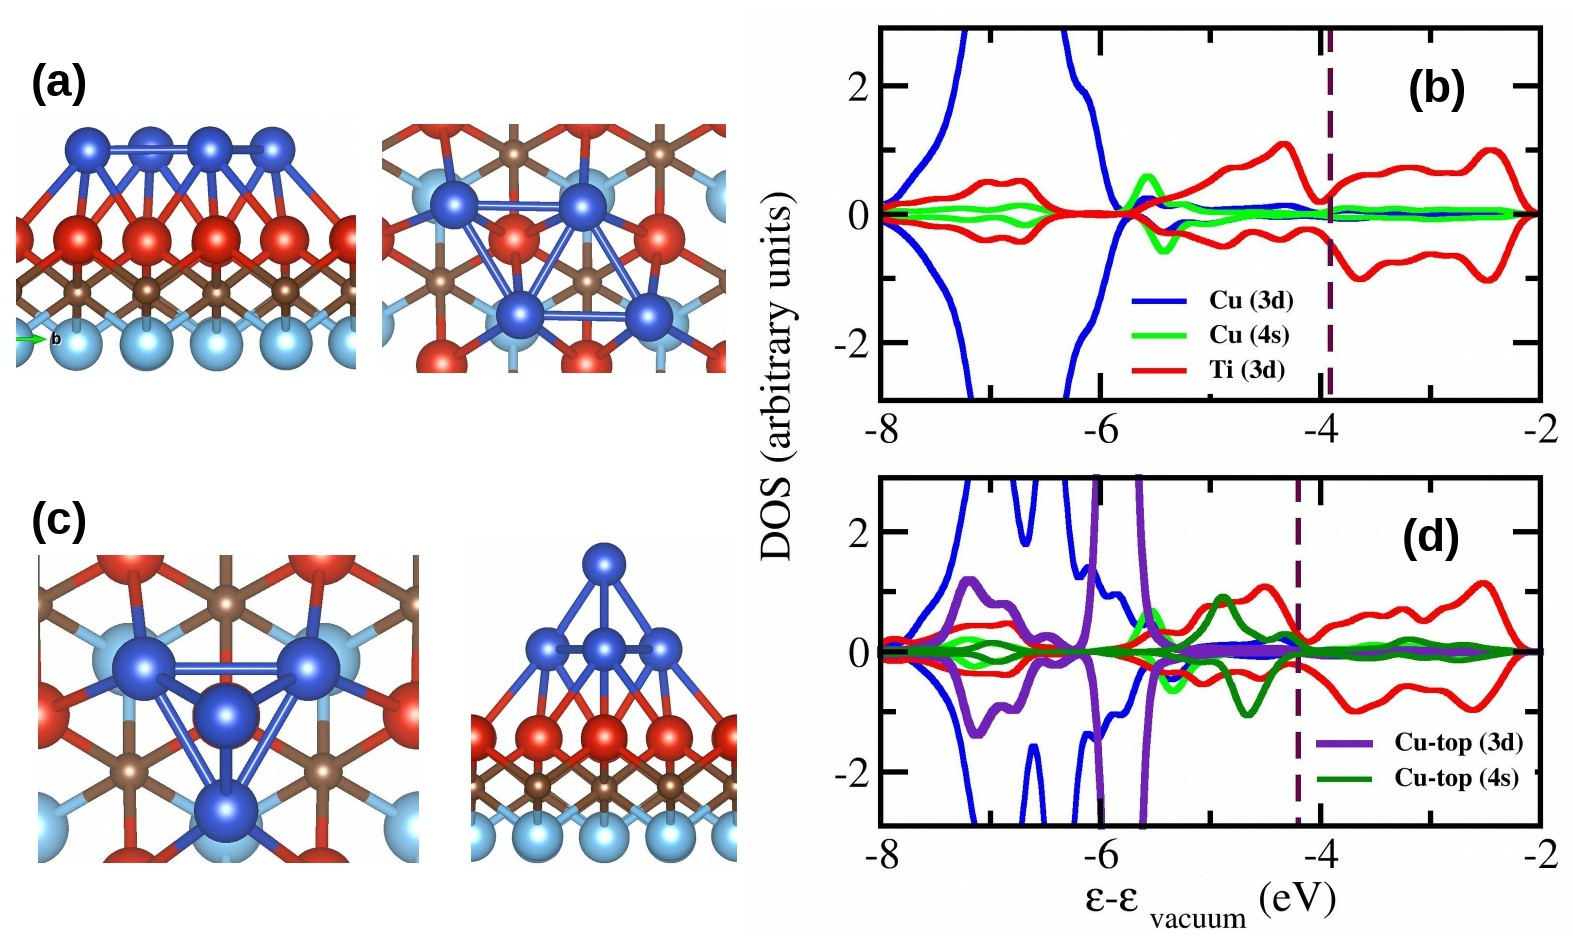
\includegraphics[width=12cm]{./Appendix2/Appendix2_figures/cu_ti2c.jpg} \\[0cm]
 \end{center}
 \caption{Side view and top view of Cu$_4$ supported on Ti$_2$C (Cu$_4$/Ti$_2$C) in (a) rhombus and (c) tetrahedral geometry. (c) and (d) shows the partial DOS projected on the
 Ti-$d$ and Cu-$d$ and $s$ states of rhombus-Cu$_4$/Ti$_2$C and tetrahedral-Cu$_4$/Ti$_2$C
 respectively.}
  \label{cu_ti2c}
\end{figure}


The DOS projected on the $d$-states of Cu and Ti and the $s$-states of Cu are shown in 
Figure~\ref{cu_ti2c}(b) and (d).
For both the configurations we find that at the Fermi energy the DOS is dominated
by contributions coming primarily from the Ti-$d$ states of the support, with very
small contributions coming from the Cu states. This suggests that if these supported clusters are used for catalytic 
purposes then the reactions will happen primarily on the support than on the clusters.
In case of the rhombus, the dominant contribution to the DOS from the Cu atoms can be observed 
below -5.00 eV. 
In contrast, we observe that there are Cu states (from the Cu atom not interacting
with the substrate) near the Fermi energy in case of the tetrahedron (Figure~\ref{cu_ti2c}(d)). Compared to the gas phase clusters, we find
that on Ti$_2$C, all the $s$ states are also occupied suggesting transfer 
of electrons from the support to the clusters, which is consistent with the fact that Cu
is more electronegative than Ti. The direction of charge transfer is further 
corroborated by the charge density difference plots shown in Figure S2 of SI where we observe accumulation (depletion) of charges on (from) the Cu (Ti) atoms. From the Bader charge analysis we find that there is an accumulation of 2.02e (1.68e) on the rhombus (tetrahedron).
However, the charges are not uniformly distributed on the cluster. On the rhombus, each of
the Cu atoms that form the long (short) diagonal have a charge of -0.64e (-0.37e).
In case of the tetrahedron, each of the Cu atoms interacting with the surface have a
negative charge of 0.46e. The one on the vertex have a charge of -0.30e.

\noindent \textit{Copper cluster supported on Ti$_2$CO$_2$:} To determine the lowest energy configuration
of the tetramer on the oxygen terminated surface, we considered several
possible configurations. Those are shown in Figure S5  of SI. The most
stable configurations of the rhombus and the tetrahedron is shown in
Figure~\ref{cu_ti2co2}(a) and (c) respectively. In contrast with the pristine surface,
in this case, we find that
the 3D tetrahedral configuration of the cluster is lower in energy
than the 2D rhombus by about 0.62 eV. The adsorption
energy of the tetrahedral cluster is about -0.66 eV/Cu atom, which
is about one-third of the value observed for the same on the pristine surface.
Additionally, unlike that of the pristine surface where the Cu atoms occupy
the hollow site, here the Cu atoms are almost on top of the O atoms. As a
consequence the Cu-Cu bond lengths of the supported clusters are only
slightly elongated compared to their gas phase bond lengths. For example,
for the tetrahedra, the gas phase Cu-Cu bond lengths are 2.42 \AA, while
on Ti$_2$CO$_2$ the Cu-Cu bond lengths of the Cu atoms interacting with O
(apical Cu atom interacting with those at the base) are 2.45 (2.42) \AA. 

In order to understand for the preference of the tetrahedral configuration,
we have computed the adsorption energy of a Cu adatom on this surface. In
contrast with the pristine surface we find that $E_{ads}^1$ is -1.58 eV/Cu atom.
This energy is comparable with the binding energy of the clusters in the
gas phase suggesting that the preference between a 2D and 3D structure depends
on the subtle balance between the two energies. For the rhombus, two
types of Cu-O bond are observed, a pair of shorter ones (each 1.91 \AA~long) involving the Cu atoms
forming the long diagonal of the rhombus and two longer ones (each 1.97 \AA) involving the other two Cu atoms. In contrast for the tetrahedron, all the three
Cu-O bonds are of equal length (each 1.89 \AA) and are smaller than that observed in case of rhombus. This suggests that the interaction of the tetrahedron
with the surface is stronger than that of the rhombus, which is corroborated by the interaction energies ($E_{int}$) of -1.14 eV/Cu atom for the tetrahedron versus that of -0.76 eV/atom for the rhombus. This interaction weakens the Cu-Cu bonds between the Cu atoms that are interacting with the surface. However, this energy cost can be compensated in case of the tetrahedron, where the fourth Cu atom occupies the hollow site formed by the other three Cu atoms. As a result in this case the tetrahedron is stabilized more than the rhombus resulting in change from a 2D to a 3D configuration of the cluster on Ti$_2$CO$_2$.


\begin{figure}[ht]
 \begin{center}
    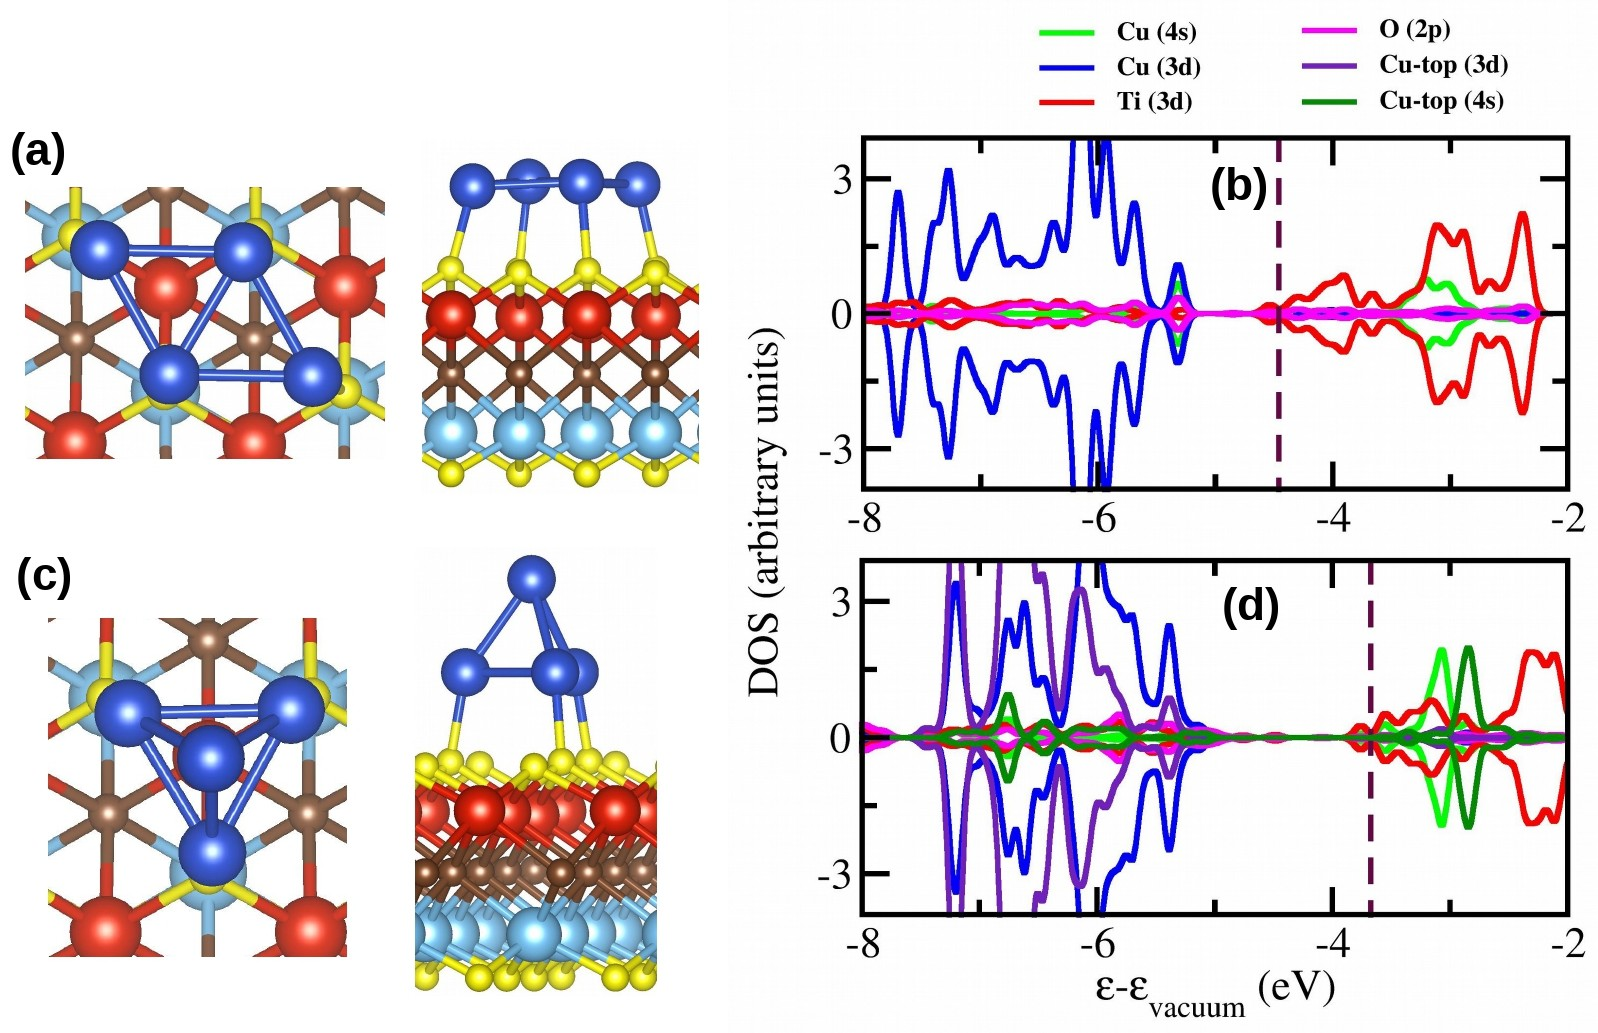
\includegraphics[width=12cm]{./Appendix2/Appendix2_figures/cu_ti2co2.jpg} \\[0cm]
 \end{center}
 \caption{Side view and top view of Cu$_4$ supported on Ti$_2$C (Cu$_4$/Ti$_2$CO$_2$) in (a) rhombus and (c) tetrahedral geometry. (c) and (d) shows the partial DOS projected on the
 Ti-$d$, Cu-$d$ and $s$ and O-$p$ states of rhombus-Cu$_4$/Ti$_2$CO$_2$ and tetrahedral-Cu$_4$/Ti$_2$CO$_2$
 respectively.}
  \label{cu_ti2co2}
\end{figure}

Figure~\ref{cu_ti2co2}(b) and (d) shows the density of states of the cluster
and the support. We find that both the clusters are non-magnetic. The Cu-$d$
states that have overlaps with the O-$p$ states occur below -5.0 eV and are
occupied. Additionally, we observe empty Cu-$s$ states above the Fermi energy
that is indicative of the fact that the clusters loose electrons. These electrons
primarily fill up the O-$p$ states that in turn pushes electrons back to the
Ti-$d$ states, which were occupying the O-$p$ states in absence of the clusters
(Figure~\ref{fig:1}(d)). This results in partial occupancy of the empty Ti-$d$
states, thereby shifting the Fermi energy to the bottom of the conduction band that are primarily from Ti-$d$ states. From Bader charge analysis we find that
each of the clusters have +1.43e charge. On both the clusters the charge distribution on the atoms are not uniform. On the rhombus the Cu atoms that are
strongly bound to the O atom and form the long diagonal have a charge of +0.58e each while the other two Cu atoms have a charge of +0.15e each. Similarly, for the tetrahedron, while the Cu atoms interacting with the O atoms have a charge of +0.48e each, the fourth Cu on the vertex is neutral. We note that in a previous DFT based study of CO$_2$ adsorption on Cu clusters supported on TiO$_2$ by Iyemperumal \textit{et al.}, they have shown that a charge of around +0.5e
on the Cu atoms indicates that they are in the +2 oxidation state while those having a charge of about
+0.2e belongs to +1 oxidation state. Zero charge on the Cu atom indicates that it is in zero oxidation state
\cite{iyemperumal2017activation}. Based on their
classification, we find that for the rhombus on the Ti$_2$CO$_2$, two of the Cu atoms
are in +1 oxidation state and the remaining two are in +2 oxidation state. In contrast,
in the supported tetrahedra, three of the Cu atoms are in +2 oxidation state and the
fourth one is in 0 oxidation state.


\subsection{CO\texorpdfstring{$_2$}{} adsorption on supported Cu tetramer}

\noindent The first step towards reduction of CO$_2$ is its capture and activation. Neutral CO$_2$ is highly stable and has a linear geometry in its ground state. Each
C-O bond length is 1.17 \AA. Upon chemisorption, it undergoes an one electron reduction
to form CO$_2$ anion, the latter having a bent geometry. This bent configuration is also
known to be highly active. How CO$_2$ interacts with a catalyst not only depends on the 
catalyst structure but also the charge on it. In this section we have studied the 
adsorption of CO$_2$ on Cu$_4$ (both planar and tetrahedral configurations)
supported on Ti$_2$C (the cluster becomes negatively charged) and Ti$_2$CO$_2$ (the 
cluster becomes positively charged) to elucidate the effect of the cluster geometry, charge and 
interaction of support on the adsorption of CO$_2$.


\begin{table}
 
 \label{tab:04}
  \begin{center}
   
    \begin{tabular}{|*{8}{c|}}
    \hline
  Cluster & CO$_2$ & $\Delta E$ & $\Delta q$ & $E_{ads}$ & $E_{int}$ & $E_{def}^{CO_2}$& $E_{def}^{Cu_{4}/Ti_{2}C}$\\
         geometry          &        geometry         & (eV) & (e) & (eV) & (eV) & (eV) & (eV) \\
    \hline
    rhombus   &  linear  & 0.00 & -0.05 & -0.17 & -0.17 & 0.00 & 0.00\\
    \hline
    rhombus & bent & 0.18 & -1.06 & 0.01 & -3.39 & 3.01 & 0.39 \\
    \hline
    tetrahedron & linear & 1.28 & -0.06 & -0.16 & -0.17 & 0.00 & 0.01 \\
    \hline
    tetrahedron & bent & 1.42 & -0.56 & -0.04 & -1.62 & 1.33 & 0.25 \\
 %     CO$_2$-Cu$_4$/Ti$_2$CO$_2$ & \multicolumn{1}{c|}{rel.$E$}
%		    & \multicolumn{1}{c|}{$E^{CO{_2}}_{bind}$} 
%		    & \multicolumn{1}{c|}{$E^{CO{_2}}_{int}$ }
%		    & \multicolumn{1}{c|}{$d^{av}_{CO}$ }
%			& \multicolumn{1}{c|}{$\angle{OCO}$}
%			& \multicolumn{1}{c|}{$q$ } \\
%			&(eV)&(eV)&(eV)&(\AA)&($^{\circ}$)&(e$^-$) \\
			\hline 
			  



%l-rhombus     &0.42&-0.41&-0.46&1.17&177.2&-0.01\\ \hline
%nl-rhombus    &0.10&-0.73&-5.23&1.32&118.1&-1.14\\ \hline
%l-tetrahedron &0.00&-0.46&-0.50&1.17&176.8&-0.01\\  \hline
%nl-tetrahedron  &0.40&-0.06&-1.09&1.22&146.1&-0.46\\ \hline
  \end{tabular}
  \end{center}
  \caption{Relative energy ($\Delta E$), amount of charge on CO$_2$ ($\Delta q$), adsorption energy ($E_{ads}$),
  interaction energy ($E_{int}$) and deformation energies ($E_{def}^i$) of CO$_2$ on copper tetramers supported on Ti$_2$C.}
\end{table} 


%\begin{table}
 %\caption{Adsoprtion of linear (l) and bent (nl) CO$_2$ on rhombus and tetrahedral geometry of copper tetramer supported on pritine Ti$_2$C (Cu$_4$/Ti$_2$C).}
 %\label{tab:04}
  %\begin{center}
   
   % \begin{tabular}{|*{7}{c|}}
  
    %\hline
     % CO$_2$-Cu$_4$/Ti$_2$C & \multicolumn{1}{c|}{rel.$E$}
	%	    & \multicolumn{1}{c|}{$E^{CO{_2}}_{bind}$} 
	%	    & \multicolumn{1}{c|}{$E^{CO{_2}}_{int}$ }
	%	    & \multicolumn{1}{c|}{$d^{av}_{CO}$ }
	%		& \multicolumn{1}{c|}{$\angle{OCO}$}
	%		& \multicolumn{1}{c|}{$q$ } \\
	%		&(eV)&(eV)&(eV)&(\AA)&($^{\circ}$)&(e$^-$) \\
	%		\hline 
	%		  



%l-rhombus     &0.00&-0.17&-0.17&1.17&179.5&-0.05\\ \hline
%nl-rhombus    &0.18& 0.01&-3.39&1.28&121.84&-1.06\\ \hline
%l-tetrahedron  &1.28&-0.16&-0.17&1.17&179.2&-0.06\\ \hline
%nl-tetrahedron &1.42&-0.04&-1.62&1.22&139.8&-0.56\\ \hline

%  \end{tabular}
  
%  \end{center}
%\end{table} 

\subsubsection{CO\texorpdfstring{$_2$}{} on Cu\texorpdfstring{$_4$}{}/Ti\texorpdfstring{$_2$}{}C}

On both the negatively charged clusters we have tried several possible 
CO$_2$ adsorption configurations (both linear and bent), relaxed geometries of which are given in 
Figure S6  and Figure S7 of SI. 

Figure~\ref{co2_ti2c} shows the most stable configurations of CO$_2$
adsorbed on the rhombus and tetrahedral clusters on Ti$_2$C in linear and bent adsorption
geometries. We find that in the linear configuration (Figure~\ref{co2_ti2c}(a) and (c)), irrespective of the shape of the cluster, CO$_2$ binds weakly with binding energies of -0.17 and -0.16 eV on the rhombus and the tetrahedron respectively. For the rhombus, the Cu-O$_{CO_2}$ distances are about 3.02 and 3.09~\AA~while on the tetrahedra they are about 3.20 \AA. For both the cases the CO$_2$ bond lengths and bond angles remain similar to that 
observed in the gas phase.


\begin{figure}[ht]
 \begin{center}	
    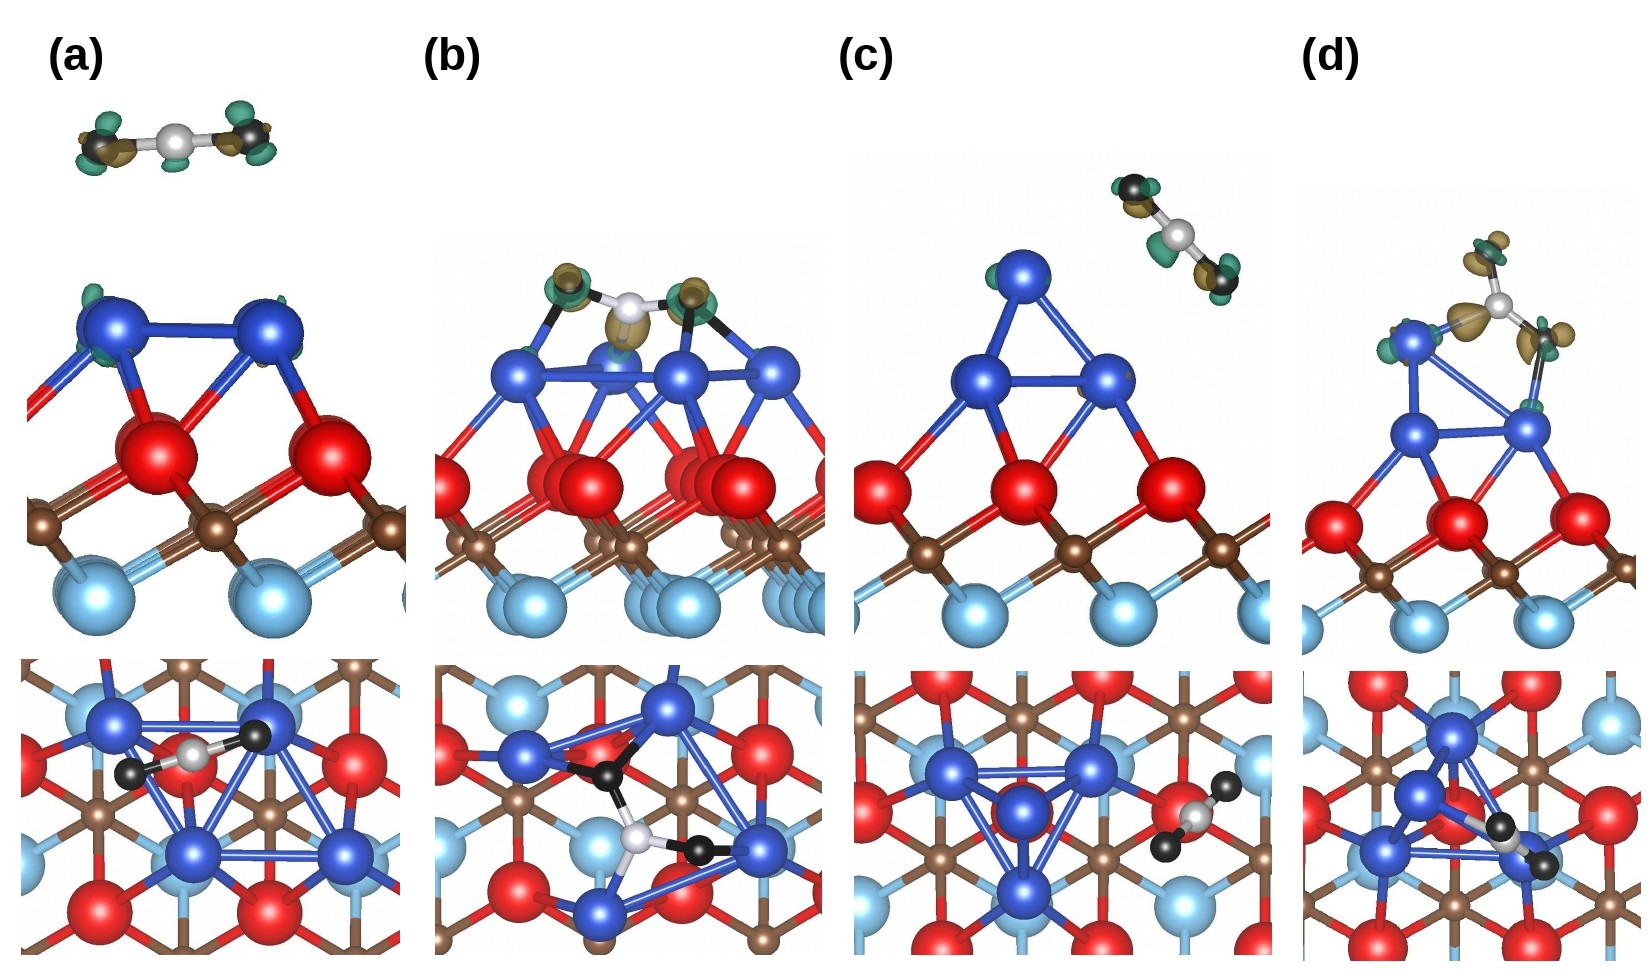
\includegraphics[width=13cm]{./Appendix2/Appendix2_figures/figure7.jpg} \\[0cm]
 \end{center}
 \caption{Most stable CO$_2$ adsorption configurations on copper tetramer supported on pristine Ti$_2$C: (a) linear and (b) bent configurations of CO$_2$ adsorbed on rhombus-Cu$_4$(2D)/Ti$_2$C respectively.
 (c) linear (d) bent configurations of CO$_2$ adsorbed on tetrahedral Cu$_4$(3D)/Ti$_2$C respectively.
 In this and the following figures the C and O atoms of CO$_2$ are represented by grey and black spheres
 respectively.
 Also shown are the charge transfer isosurfaces with isovalues of (a) 0.006, (b) 0.193, (c)0.006 and
 (d) 0.101 electron/Å$^3$. The caramel (fern) isosurfaces show charge accumulation (depletion).}
  \label{co2_ti2c}
\end{figure}

The bent CO$_2$ shows an endothermic adsorption on the supported rhombus with an adsorption energy of 0.01 eV (Figure~\ref{co2_ti2c}(b)). The C of CO$_2$ binds to one of the Cu atoms that form the short diagonal of the rhombus and has less negative charge. The two O atoms
bind to the Cu atoms that form the long diagonal. The Cu-O$_{CO_2}$ bond lengths are about 2.10 \AA~while
the Cu-C$_{CO_2}$ bond length is about 2.00 \AA. We find that 1.06e charge is 
transferred from the cluster to CO$_2$. The OCO bond angle is 121.84$^{\circ}$ with C-O
bond lengths of 1.30 and 1.27 \AA~respectively. In this adsorption geometry, we find that the interaction
energy between the bent CO$_2$ and the distorted cluster is about -3.39 eV. However, the energy gained
through this interaction is used in the deformation of CO$_2$ (deformation energy of 3.01 eV) and the cluster
(deformation energy of 0.39 eV). As a result the overall adsorption is weakly endothermic with an
adsorption energy of 0.01 eV.

In addition to the above configuration, we find another configuration (about 5 meV higher in energy than
the previous one) in which the CO$_2$ molecule binds to the Cu atom of the rhombus through the C atom and the O atoms point away from the surface (Figure S6(e) in SI). The Cu-C distance is about 2.21 \AA. We find that about 0.60e charge is transferred from the cluster to the carbon dioxide molecule, with most of the transferred charge accumulated on the C atom. The O$_{CO_2}$CO$_{CO_2}$ bond angle is reduced to 142.74$^{\circ}$ and each of the C-O$_{CO_2}$ 
bonds are elongated to 1.23 \AA. Additionally the cluster is also distorted with elongation of the Cu-Cu bonds. The energy cost for the distortion of the Cu cluster on support (0.06 eV) and the bending of the CO$_2$ molecule (1.15 eV) is slightly higher than the energy gain by the CO$_2$ interaction (-1.20 eV), thereby making the overall process endothermic.

On the tetrahedral cluster, we find the adsorption of the bent CO$_2$ to be weakly exothermic (-0.04 eV). As shown in Figure~\ref{co2_ti2c}(d), the C atom binds to the Cu atom at the vertex of the tetrahedra while one of the O atoms bind to a Cu atom that is interacting with the surface. One of the C-O$_{CO_2}$ bonds (for the C and O atoms interacting with the cluster) is elongated to 1.24 \AA, while the other one is elongated to 1.21 \AA. The O$_{CO_2}$CO$_{CO_2}$ bond angle is 139.8$^{\circ}$. The charge transfer plot shows that for this case about 0.56e are transferred to the CO$_2$ molecule. Here also we observe significant charge accumulation on the C atom. Similar to the case of the rhombus, the cluster is highly distorted; the energy cost to distort the cluster and bend the CO$_2$ molecule is significantly large. However, compared to the rhombus, in this case the energy cost for distortion is slightly smaller than the energy gained from the interaction of CO$_2$ with the cluster results. Hence the overall adsorption process is exothermic.

\subsubsection{CO\texorpdfstring{$_2$}{} on Cu\texorpdfstring{$_4$}{}/Ti\texorpdfstring{$_2$}{}CO\texorpdfstring{$_2$}{}}
\label{fooking}

\begin{table}
 
 \label{tab:05}
  \begin{center}
   
    \begin{tabular}{|*{8}{c|}}
    \hline
  Cluster & CO$_2$ & $\Delta E$ & $\Delta q$ & $E_{ads}$ & $E_{int}$ & $E_{def}^{CO_2}$& $E_{def}^{Cu_{4}/Ti_{2}CO_{2}}$\\
         geometry          &        geometry         & (eV) & (e) & (eV) & (eV) & (eV) & (eV) \\
    \hline
    rhombus   &  linear  & 0.42 & -0.01 & -0.41 & -0.46 & 0.01 & 0.04\\
    \hline
    rhombus & bent & 0.10 & -1.14 & -0.73 & -5.23 & 3.71 & 0.79 \\
    \hline
    tetrahedron & linear & 0.00 & -0.01 & -0.46 & -0.50 & 0.01 & 0.03 \\
    \hline
    tetrahedron & bent & 0.40 & -0.46 & -0.06 & -1.09 & 0.96 & 0.07 \\
 %     CO$_2$-Cu$_4$/Ti$_2$CO$_2$ & \multicolumn{1}{c|}{rel.$E$}
%		    & \multicolumn{1}{c|}{$E^{CO{_2}}_{bind}$} 
%		    & \multicolumn{1}{c|}{$E^{CO{_2}}_{int}$ }
%		    & \multicolumn{1}{c|}{$d^{av}_{CO}$ }
%			& \multicolumn{1}{c|}{$\angle{OCO}$}
%			& \multicolumn{1}{c|}{$q$ } \\
%			&(eV)&(eV)&(eV)&(\AA)&($^{\circ}$)&(e$^-$) \\
			\hline 
			  



%l-rhombus     &0.42&-0.41&-0.46&1.17&177.2&-0.01\\ \hline
%nl-rhombus    &0.10&-0.73&-5.23&1.32&118.1&-1.14\\ \hline
%l-tetrahedron &0.00&-0.46&-0.50&1.17&176.8&-0.01\\  \hline
%nl-tetrahedron  &0.40&-0.06&-1.09&1.22&146.1&-0.46\\ \hline
  \end{tabular}
  \end{center}
  \caption{Relative energy ($\Delta E$), amount of charge on CO$_2$ ($\Delta q$), adsorption energy ($E_{ads}$),
  interaction energy ($E_{int}$) and deformation energies ($E_{def}^i$) of CO$_2$ on copper tetramers supported on Ti$_2$CO$_2$.}
\end{table} 

Analogous to that of Cu$_4$/Ti$_2$C, here also we explored several geometries of CO$_2$ adsorbed on the clusters in the linear and bent form. These are shown in Figure S8 and Figure S9 of SI.

In their lowest energy configurations, the linear CO$_2$ shows an exothermic adsorption 
on both the tetrahedral ($E_b^{CO_2}=$ -0.46 eV) and rhombus ($E_b^{CO_2}=$ -0.41 eV) 
clusters with the former slightly more stronger than the latter. We note that this is 
stronger than the binding energy of the linear CO$_2$ molecule on these clusters when they are on Ti$_2$C. 
The relaxed geometries for the same are shown in 
Figure~\ref{co2_ti2co2}(a) and (c). On the 2D rhombus, the linear CO$_2$ molecule binds 
to one of the Cu atoms having larger positive charge through 
the O atom of the CO$_2$ molecule (Figure~\ref{co2_ti2co2}(a)). The Cu-O$_{CO_2}$ bond 
length is about 2.17 \AA. The C-O$_{CO_2}$ bond between the C and O atoms of CO$_2$
that are interacting with the Cu cluster is slightly elongated to 1.18 \AA~while the 
other C-O$_{CO_2}$ bond length is 1.16 \AA. The O$_{CO_2}$CO$_{CO_2}$ bond angle is 
177.2$^{\circ}$. On the tetrahedral cluster (Figure~\ref{co2_ti2co2}(c)) the linear 
CO$_2$ molecule binds to the Cu atom interacting with the surface O atom through one of 
its O$_{CO_2}$ atom with a Cu-O$_{CO_2}$ bond length of about 
2.17 \AA. The C-O$_{CO_2}$ bond (that interacting with the cluster) is slightly 
elongated to 1.18 \AA, while the other one is shortened to 1.16 \AA. The 
O$_{CO_2}$CO$_{CO_2}$ bond angle is about 176.8$^{\circ}$. In both the cases we observe 
negligible charge transfer. 

\begin{figure}[ht]
 \begin{center}	
    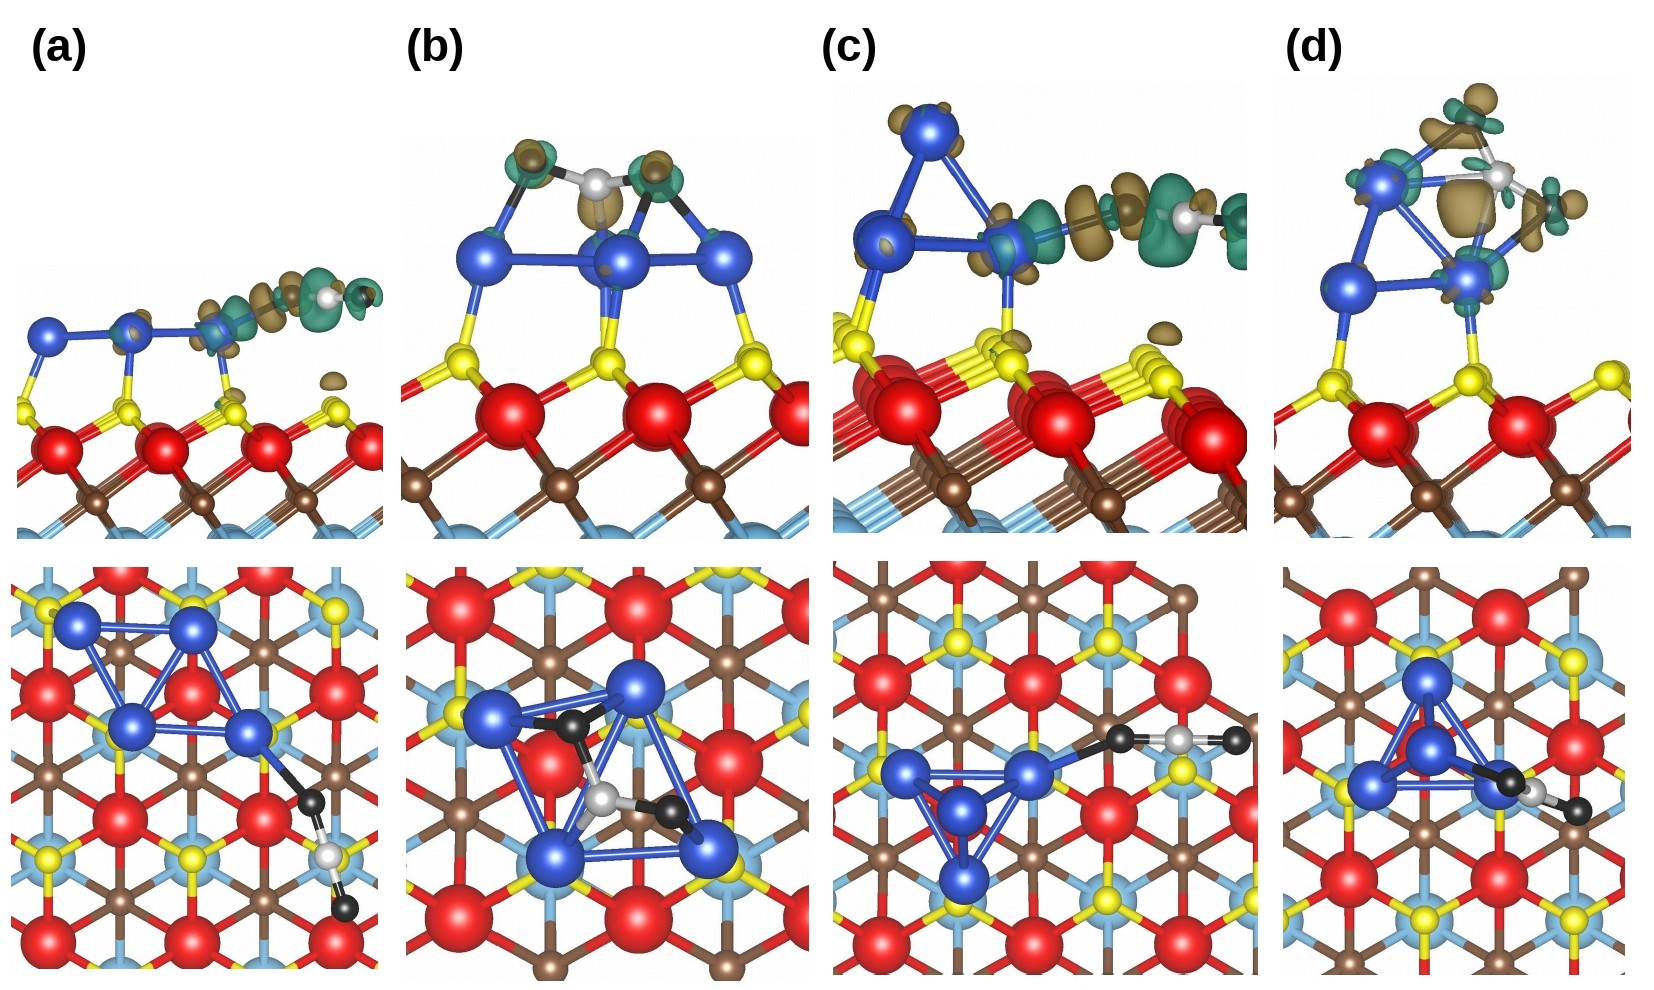
\includegraphics[width=12cm]{./Appendix2/Appendix2_figures/figure8.jpg} \\[0cm]
 \end{center}
 \caption{Most stable CO$_2$ adsorption configurations on copper tetramer supported on pristine Ti$_2$CO$_2$: (a) linear and (b) bent configurations of CO$_2$ adsorbed on rhombus-Cu$_4$(2D)/Ti$_2$CO$_2$ respectively.
 (c) linear (d) bent configurations of CO$_2$ adsorbed on tetrahedral Cu$_4$(3D)/Ti$_2$CO$_2$ respectively.
 Also shown are the charge transfer isosurfaces with isovalues of (a) 0.014, (b) 0.202, (c) 0.014 and
 (d) 0.047 electron/Å$^3$. The caramel (fern) isosurfaces show charge accumulation (depletion).}
  \label{co2_ti2co2}
\end{figure}
 
Unlike that of Ti$_2$C, the adsorption of bent CO$_2$ on both the clusters supported on Ti$_2$CO$_2$ are exothermic in nature. The CO$_2$ adsorption energy on the tetrahedron
is about -0.06 eV. The relaxed geometry is shown in Figure~\ref{co2_ti2co2}(d). On the 3D cluster the O$_{CO_2}$CO$_{CO_2}$ bond angle is reduced to 146.1$^{\circ}$.
Both the CO$_{CO_2}$ bond lengths are elongated to 1.22 \AA. The C is closer to the basal Cu atom (Cu-C bond length 2.13 \AA) and the Cu-O$_{CO_2}$ bond lengths are about 2.13 \AA. Bader charge analysis shows that
the CO$_2$ molecule gains about 0.46e. 

The lowest energy configuration of the bent CO$_2$ on the rhombus is shown in Figure~\ref{co2_ti2co2}(b). In contrast to all the other cases of CO$_2$ adsorption considered
in this study, the binding of CO$_2$ on this cluster shows the largest exothermicity with an
adsorption energy of -0.73 eV. In comparison with the tetrahedral configuration we find that the 
rhombus is significantly distorted upon adsorption of CO$_2$. The O$_{CO_2}$CO$_{CO_2}$ plane makes an angle of 66.2 $^{\circ}$ with the surface. The C atom binds to the Cu atom that is less positive with a Cu-C bond length of 1.90 \AA. The 
O$_{CO_2}$CO$_{CO_2}$ bond angle is drastically reduced to 118.1$^{\circ}$. The  O$_{CO_2}$-C bonds are asymmetrically elongated. Of the two O atoms of CO$_2$, the one that is bound to two Cu atoms with O$_{CO_2}$-Cu distances of about 2.01 \AA~have a 
CO$_{CO_2}$ bond length of about 1.35\AA. The second O that binds with one Cu (having 
larger positive charge) have a C-O$_{CO_2}$ bond length of about 1.29 \AA. For this 
particular case the CO$_2$ gains about 1.14e forming a highly activated CO$_2$ anion.

\subsection{Physisorption to chemisorption barrier}

After determining the CO$_2$ adsorption geometries, in this section, we present the results for
the mechanism for transition of the adsorbed CO$_2$ from the physisorbed to chemisorbed state.
We begin by noting that on the clusters supported on pristine Ti$_2$C and the tetrahedral
cluster on Ti$_2$CO$_2$ the process is endothermic, while on the rhombus supported on
Ti$_2$CO$_2$ it is exothermic. The largest endothermiticity is observed for the case of tetrahedron
on Ti$_2$CO$_2$. The pathways along with the transition states (TS) from physisorbed to chemisorbed 
CO$_2$ for each of the cases are shown in Figure \ref{fig:neb_co2}(a-d).

On the rhombus supported on pristine Ti$_2$C (Figure \ref{fig:neb_co2}(a)), the transition happens through
a metastable state (MS) where the CO$_2$ just binds to the cluster in a bent form with one of the O atom
point upwards. As a result, in this configuration, the OCO plane is still normal to the surface.
This transition involves a barrier of 0.24 eV. In the TS, the vertical distance between the Cu
atoms and the C atom is about 1.95 \AA. The CO$_2$ molecule is activated with an OCO bond angle of 140.20$^\circ$
and CO bond lengths of about 1.25 and 1.22 \AA. The transition from the MS state to the FS involves the distortion
of the cluster to accommodate the CO$_2$ molecule in an adsorption geometry where the OCO plane is completely
horizontal. This involves a barrier of 0.12 eV. Thus, the overall barrier for physisorption
to chemisorption of CO$_2$ on this cluster is 0.36 eV.
On the tetrahedron supported on Ti$_2$C (Figure \ref{fig:neb_co2}(b)) the
barrier is about 0.17 eV. In this case also the CO$_2$ molecule is bent in the TS with OCO bond
angle of 154.71$^\circ$ and CO bond lengths of 1.20 \AA~each.

On the rhombus supported on Ti$_2$CO$_2$, the transition from physisorbed to chemisorbed CO$_2$
happens through two metastable states. The first metastable state (MS-I) (Figure \ref{fig:neb_co2}(c)) is about 0.12 eV higher in energy than the initial state (IS). In MS-I the CO$_2$ molecule remains linear and is bound
almost vertically to the Cu cluster. The OCO bond angle is 179.84$^\circ$. The CO bond lengths are
also close to those in the gas phase. The transition from IS to MS-I involves a rotation of the
CO$_2$ molecule. At the TS-1 (Figure \ref{fig:neb_co2}(c)) the Cu-O$_{CO_2}$ bond length is about 2.12 \AA. There are 
negligible changes in CO$_2$ geometry. The second metastable state (MS-II) is about 0.37 eV
lower in energy than MS-I. The path from MS-I to MS-II is associated with conversion of the
CO$_2$ molecule from linear to bent geometry. In MS-II, in addition to the O atom of CO$_2$ that
is already bound to the Cu atom, the C atom binds in a bridge configuration to the Cu atoms
that form the short diagonal of the rhombus. The OCO bond angle is 129.22$^\circ$, the other O
atom pointing away from the surface. The C-O bond length between C and O atom bound to
Cu is 1.31 \AA, while the other one is about 1.21 \AA. The Cu-O (Cu-C) bond length(s) is 
(are) 1.88 \AA~(2.16 and 2.14 \AA). In the TS-II, the CO$_2$ is still bound to the cluster
through a single Cu atom. The OCO bond angle is 161.60$^\circ$. In the final part of the path
the CO$_2$ goes from MS-II to the final chemisorbed form. This involves a barrier of 0.22 eV.
During this process the second O atom of CO$_2$ that was not bound to the cluster now
binds to the second Cu atom forming the long diagonal of the cluster resulting in the CO$_2$
molecule lying horizontally on the cluster. This is also accompanied by substantial
deformation of the cluster. The effective barrier for this path, i.e., the energy difference
between IS and TS-II is about 0.15 eV.

On the tetrahedron supported on Ti$_2$CO$_2$(Figure \ref{fig:neb_co2}(d)), during the transition from physisorbed to 
chemisorbed state, the system goes through a metastable that is about 0.23 eV higher
in energy than the IS. In this MS state the CO$_2$ is vertically above the surface. The shortest
distance between Cu and O$_{CO_2}$ is about 2.28 \AA. The molecule is still linear and have
CO bond lengths similar to that observed in the gas phase. The transition from IS to MS
is barrier less and endothermic. From this MS state, the CO$_2$
molecule goes to the FS through a TS state. The process is associated with a barrier of about 0.19 eV. In the TS, the OCO bond angle is 160.64$^\circ$. The apical Cu-O$_{CO_2}$ distance is 
about 2.37 \AA, while the distance between the second O and the Cu atom at the base is about
2.19 \AA. The C-O bonds are slightly elongated to 1.19 \AA. The effective barrier is 0.42 eV
and is the largest amongst all the cases considered in the study.

\begin{figure}[ht]
 \begin{center}	
    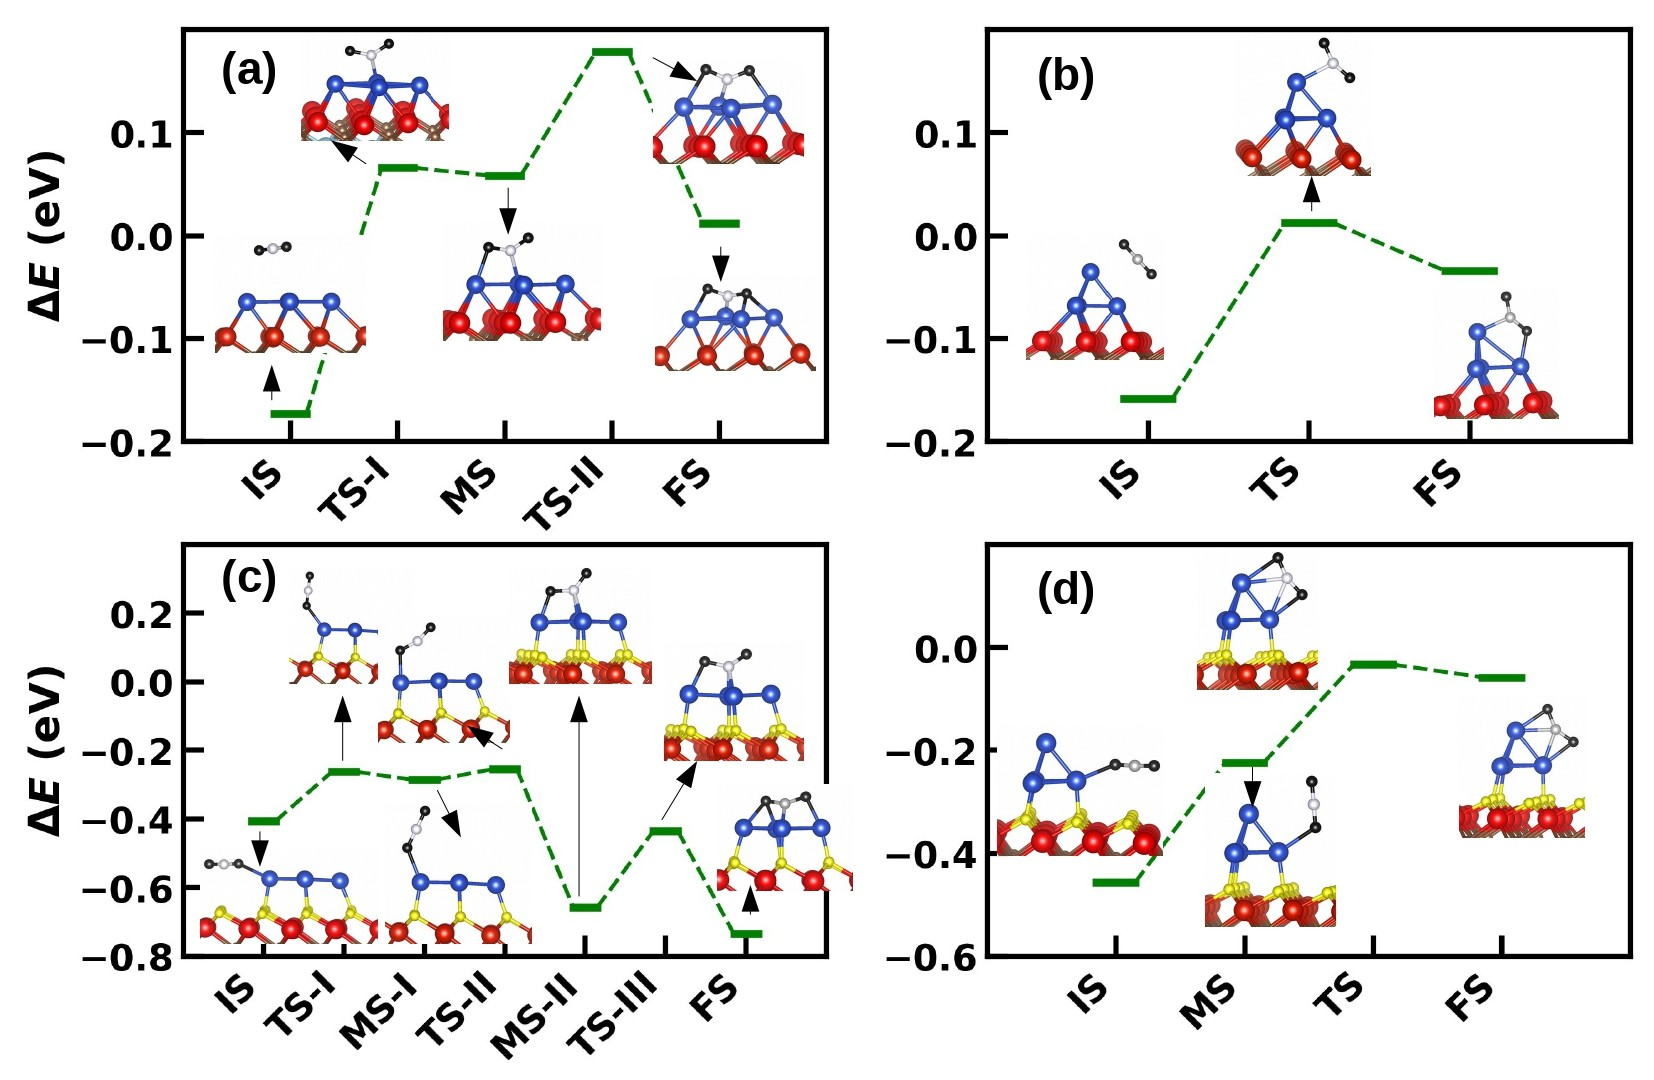
\includegraphics[width=12cm]{./Appendix2/Appendix2_figures/neb_co2.jpg} \\[0cm]
 \end{center}
 \caption{Transition of linear (physisorbed) CO$_2$ to bent (chemisorbed) one on (a) rhombus/Ti$_2$C,
 (b) tetrahedral/Ti$_2$C, (c) rhombus/Ti$_2$CO$_2$ and (d) tetrahedral/Ti$_2$CO$_2$. Also shown are
 the different IS, FS, TS and MS. ($\Delta E= E_{CO_2+Cu_4+X}-E_{Cu_{4}+X} - E^{g}_{CO_2}$) }
  \label{fig:neb_co2}
\end{figure}


\subsection{Role of charge and cluster geometry}
In order to elucidate the role of charge on the supported cluster and its geometry, we begin by noting
that on Ti$_2$C the clusters are negatively charged while on Ti$_2$CO$_2$ they are positively charged.
The magnitude of the negative charge is larger on the rhombus than on the tetrahedra. Moreover, on both
the clusters the charges on the Cu atoms are unevenly distributed. Similar features were also observed
on the positively charged clusters on Ti$_2$CO$_2$, except that the total charge on each of the clusters
are same. For these clusters this results in the Cu atoms being
in different oxidation states. On the rhombus (tetrahedra) two (three) of the Cu atoms are in Cu$^{+2}$ state while the other
two (one) are (is) in Cu$^{+1}$ (Cu$^0$) oxidation state. 

Comparing $E_{ads}$ of the chemisorbed CO$_2$ in the four cases show that CO$_2$ binds most strongly
on the positively charged rhombus. Performing an energy decomposition analysis suggests that the interaction
of the bent CO$_2$ molecule with this cluster is largest in this case ($E_{int}$=-5.23 eV). The strength
of the interaction, in decreasing order is: rhombus/Ti$_2$CO$_2$ $>$ rhombus/Ti$_2$C $>$ tetrahedron/Ti$_2$C
$>$ tetrahedron/Ti$_2$CO$_2$. This is also in accordance with the decreasing order of charge transfer from
cluster to CO$_2$ (Figure \ref{co2_int}(a)). The cause for the strongest interaction observed for rhombus/Ti$_2$CO$_2$
can be attributed to the presence of Cu atoms in their +1 and +2 oxidation state. The more electronegative O atoms 
bind to the Cu atoms in +2 oxidation state, while the C atom binds to Cu atom in +1 oxidation state.
Further, irrespective of the nature of the charge on the cluster, we find that the interaction energy
for the 2D rhombus is larger than the 3D tetrahedron. For the former case, since the cluster is flat, more
Cu atoms are exposed for interaction with CO$_2$; on the rhombus, three Cu atoms form bonds with CO$_2$ while
on tetrahedra only two Cu atoms are involved. These results suggests that for strong chemisorption of
CO$_2$ on the Cu tetramers, it is not only desirable to have 2D Cu clusters but also to have the Cu atoms
in different oxidation states, preferably in +2 and +1. The different oxidation states suggest presence
of different amount of charge on the Cu atoms. This assists in selective binding of the C and O atoms of CO$_2$
that have different electronegativities.


\begin{figure}[ht]
 \begin{center}	
    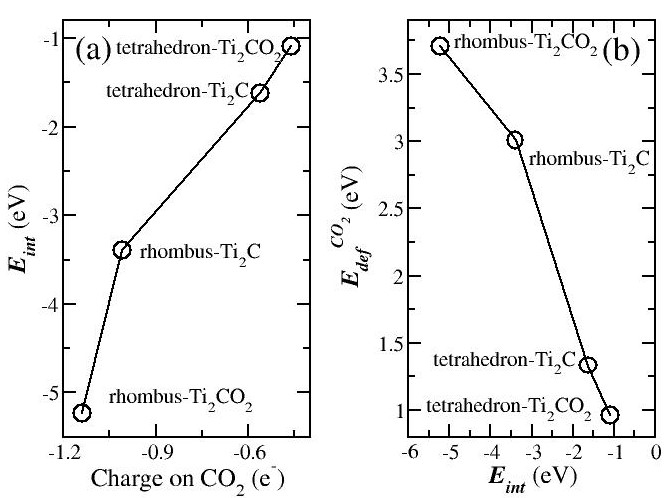
\includegraphics[width=12cm]{Appendix2/Appendix2_figures/co2_plot.jpg} \\[0cm]
 \end{center}
 \caption{(a) Variation of $E_{int}$ with charge on adsorbed CO$_2$. (b) Correlation between
 energy cost for CO$_2$ deformation ($E_{def}^{CO_2}$) and $E_{int}$. In all the cases CO$_2$ is adsorbed
 in the bent form, i.e., in chemisorbed configuration.}
  \label{co2_int}
\end{figure}

However, due to the chemisorption, there is also distortion of the cluster and the bending of the CO$_2$ molecule.
The energy needed to achieve this (energy cost) is obtained from the interaction energy. The adsorption
process will be exothermic (endothermic) if the interaction energy is larger (smaller)
than the sum of the energy cost for deforming the cluster and CO$_2$. From our calculations we find that stronger 
the interaction between the CO$_2$ and the cluster,
more bent is the CO$_2$ molecule and hence larger is the CO$_2$ deformation energy cost
(Figure \ref{co2_int}(b)). On the other
hand, the ease/difficulty with which the cluster can be deformed is also controlled by the interaction strength between
the cluster with the support. A larger interaction strength implies weakening of the Cu-Cu bonds, thereby
making the clusters more fluxional (less deformation energy cost) for CO$_2$ adsorption. This can be corroborated
upon noting the change in the Cu-Cu bond lengths in the rhombus on both the supports upon CO$_2$ adsorption
and the energy cost to undergo such deformations. On Ti$_2$CO$_2$ (Ti$_2$C), the smallest increase in the Cu-Cu bond is 0.07 \AA~(0.40 \AA) while the largest increase in the bond length is 0.59 \AA~(0.88 \AA). This
suggests that on Ti$_2$C the rhombus has to undergo a much larger distortion compared to that on Ti$_2$CO$_2$.
However, the energy cost for doing so on Ti$_2$C is almost half of that necessary on Ti$_2$CO$_2$ (0.39 eV on
Ti$_2$C vs. 0.79 eV on Ti$_2$CO$_2$), thereby indicating that the clusters on the pristine support are more
fluxional than on the O-terminated one. Thus our analysis suggests that for strong exothermic chemisorption
of CO$_2$ the Cu cluster should have the following properties: (a)  the cluster should have
a flat geometry such that all Cu atoms are accessible to the incoming CO$_2$ (b) it should be preferentially
positively charged with Cu atoms present in different oxidation states, and (c) the cluster
should be fluxional so that it can be easily deformed.

In contrast with the chemisorbed configurations, in the physisorbed ones, we find that not only the interaction
energy is same as the adsorption energy but also their magnitude is much smaller. Moreover, the deformation cost of the cluster and CO$_2$ is negligible.
This demonstrates that, indeed in these cases CO$_2$ is physisorbed on the cluster. $E_{int}$/$E_{ads}$
is larger when CO$_2$ is bound to the positively charged clusters compared to that on the negatively charged ones.
This is probably due to the fact that in the former case, the CO$_2$ molecule also interacts weakly
with the surface, thereby slightly stabilizing itself.


\section{Conclusions}
\label{concll}
In summary, we have studied CO$_2$ adsorption on 2D and 3D Cu tetramers supported on Ti$_2$C
and Ti$_2$CO$_2$ substrates. While on Ti$_2$C the cluster prefers a 2D rhombus configuration,
on Ti$_2$CO$_2$ the 3D tetrahedral configuration is more stable. Moreover, on the former (later) support
the cluster is negatively (positively) charged. From the computation of the CO$_2$ adsorption
energy and energy decomposition analysis of the same we find that for exothermic CO$_2$ chemisorption on the
cluster, the cluster should be in a 2D configuration such that the Cu atoms are exposed to the
approaching CO$_2$ molecule, highly fluxional and the Cu atoms should preferably be positively charged, having different oxidation numbers. On all the clusters that we have studied, we find that the physisorption
to chemisorption is an activated process. On most of the clusters the barrier is low except for
the tetrahedron on Ti$_2$CO$_2$ which can be attributed to the large endothermicity associated
with this process on that clusters. We hope that our study will be useful for experimentalists
and theoreticians to choose a right combination of cluster size, morphology and support for
CO$_2$ capture and reduction.

%\subsection*{Acknowledgement}
%UM acknowledges IISER Pune, India for fellowship. PG and UM acknowledges Center for Development of Advanced Computing, Pune and Param Brahma, IISER Pune, India for providing computing facilities. PG also acknowledges DST-SERB, Govt. of India, grant no:  EMR/2016/005275 and DST-Nanomission, Govt. of India, grant no: SR/NM/TP-13/2016 for funding.

\section{Supporting Information}

\begin{figure}[htb]
  \begin{center}
    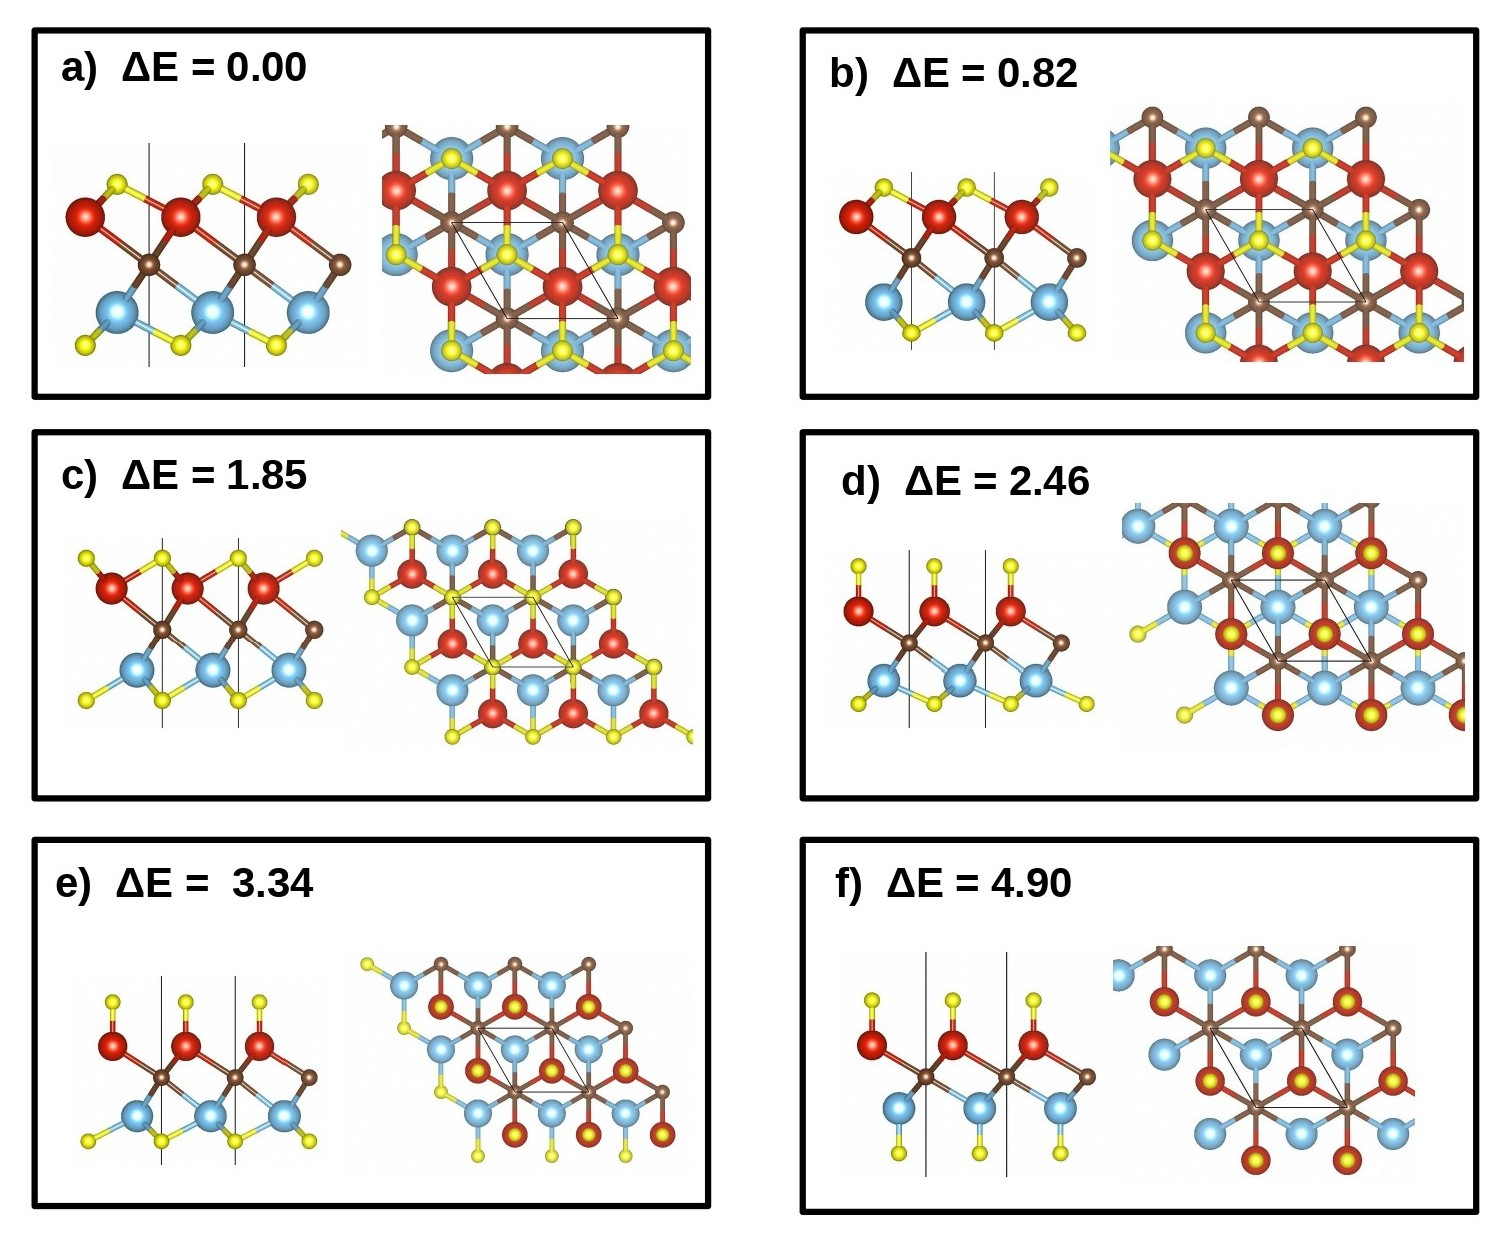
\includegraphics[width=0.9\textwidth]{./Appendix2/Appendix2_figures/photo1.jpg}
  \end{center}
    \caption{Possible isomers of O-terminations in MXene (Ti$_2$CO$_2$). $\Delta$E is the relative energy with respect to the most stable isomer. }
  \label{fig-01}
\end{figure}

\begin{figure}[htb]
  \begin{center}
    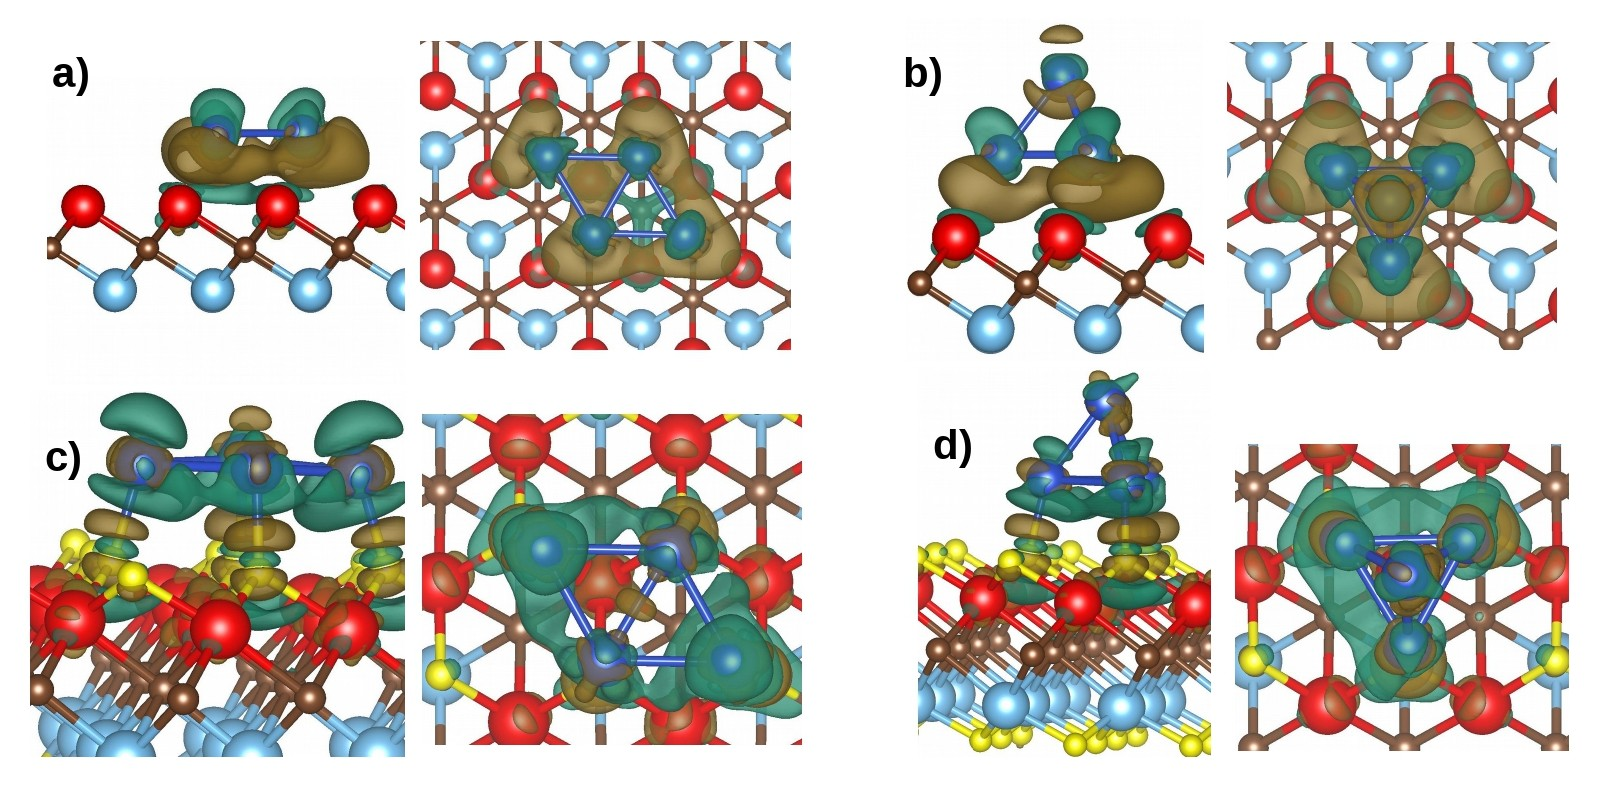
\includegraphics[width=0.9\textwidth]{./Appendix2/Appendix2_figures/figure5.jpg}
  \end{center}
\caption{Charge transfer isosurfaces of copper clusters on Ti$_2$C in (a) rhombus and (b) tetrahedral geometry and Ti$_2$CO$_2$ in (c) rhombus and (d) tetrahedral geometry. The corresponding isovalues for the isosurfaces are (a) 0.027 , (b) 0.020 , (c) 0.020  and (d) 0.020  electron/Å$^3$. The caramel (fern) isosurface show charge accumulation (depletion).}
  \label{fig-05}
\end{figure}

\begin{figure}[htb]
  \begin{center}
    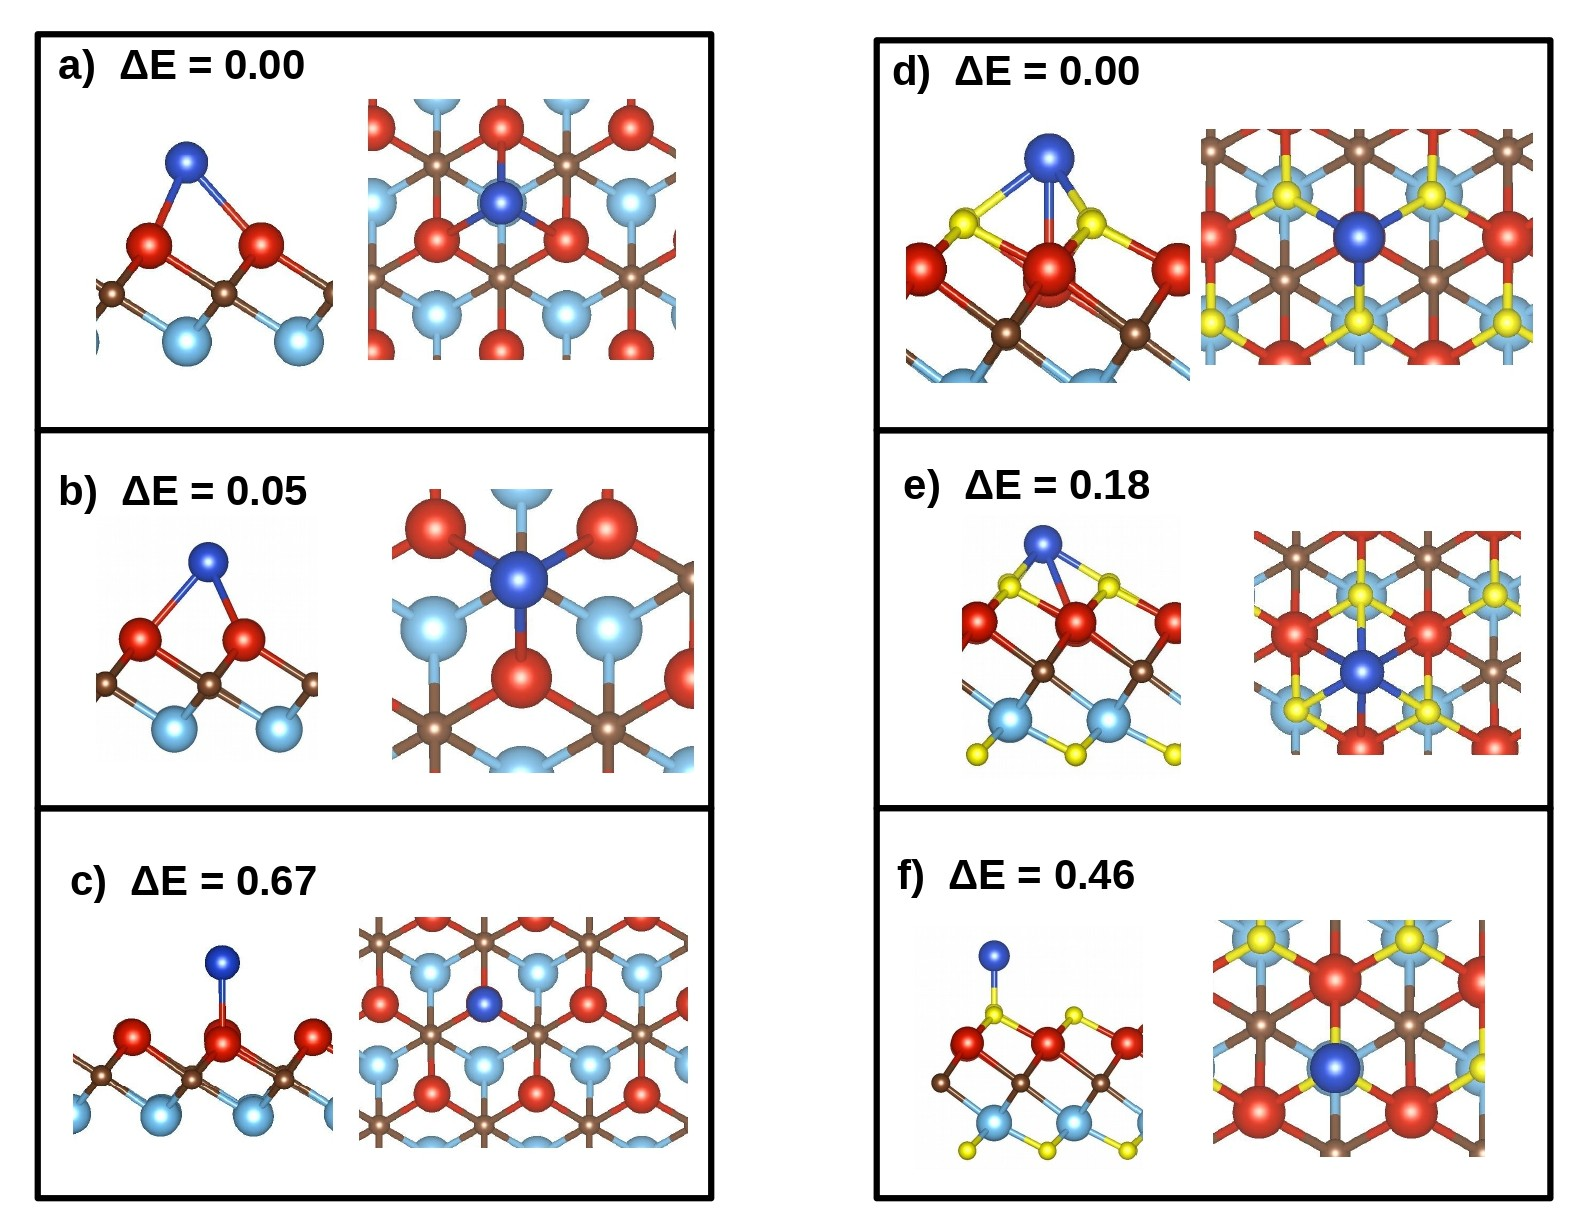
\includegraphics[width=0.8\textwidth]{./Appendix2/Appendix2_figures/photo2.jpg}
  \end{center}
    \caption{Possible adatom configurations on pristine (Cu$_1$/Ti$_2$C : [a-c]) and O-terminated (Cu$_1$/Ti$_2$CO$_2$ : [d-f]) MXene. $\Delta$E is the relative energy with respect to the most stable adatom isomer for the pristine and O-t case separately.}
  \label{fig-02}
\end{figure}


\begin{figure}[htb]
  \begin{center}
    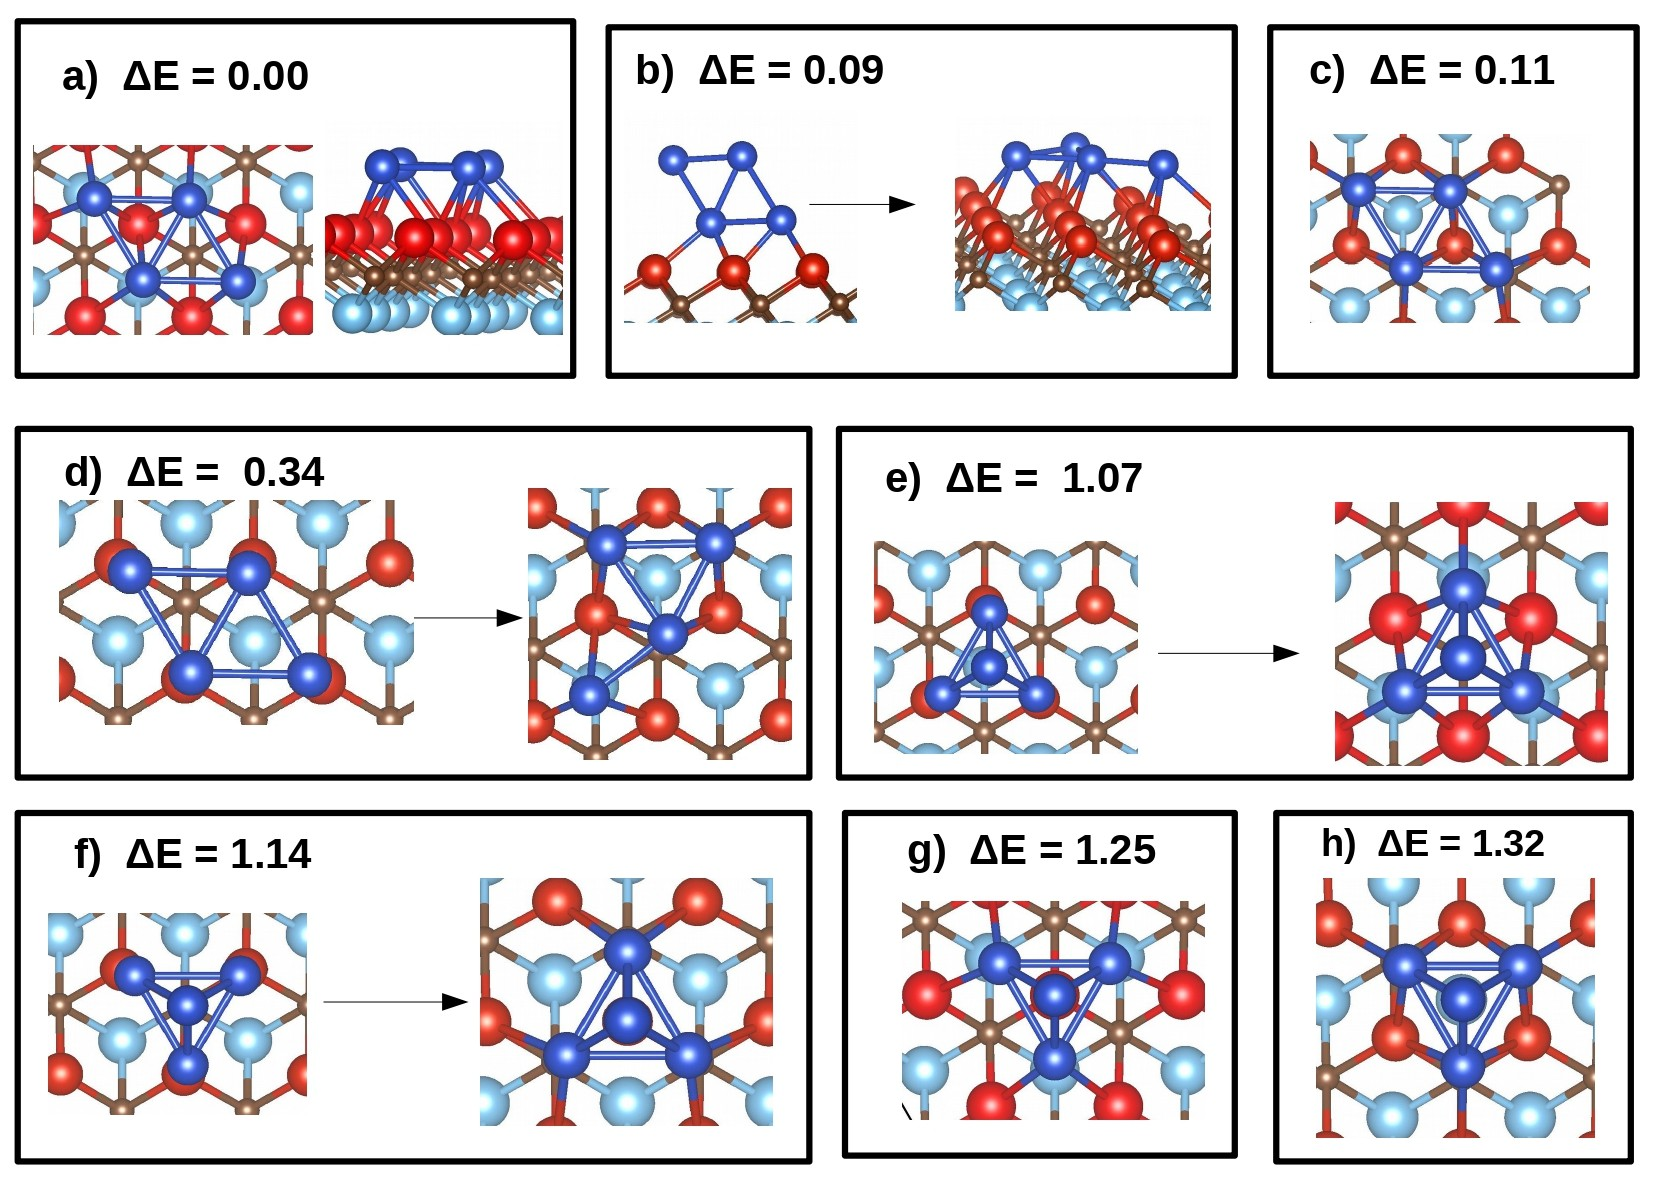
\includegraphics[width=0.9\textwidth]{./Appendix2/Appendix2_figures/photo5.jpg}
  \end{center}
    \caption{Possible tetramer configurations on pristine MXene (Cu$_4$/Ti$_2$C). $\Delta$E is the relative energy with respect to the most stable isomer.}
  \label{fig05}
\end{figure}

\begin{figure}[htb]
  \begin{center}
    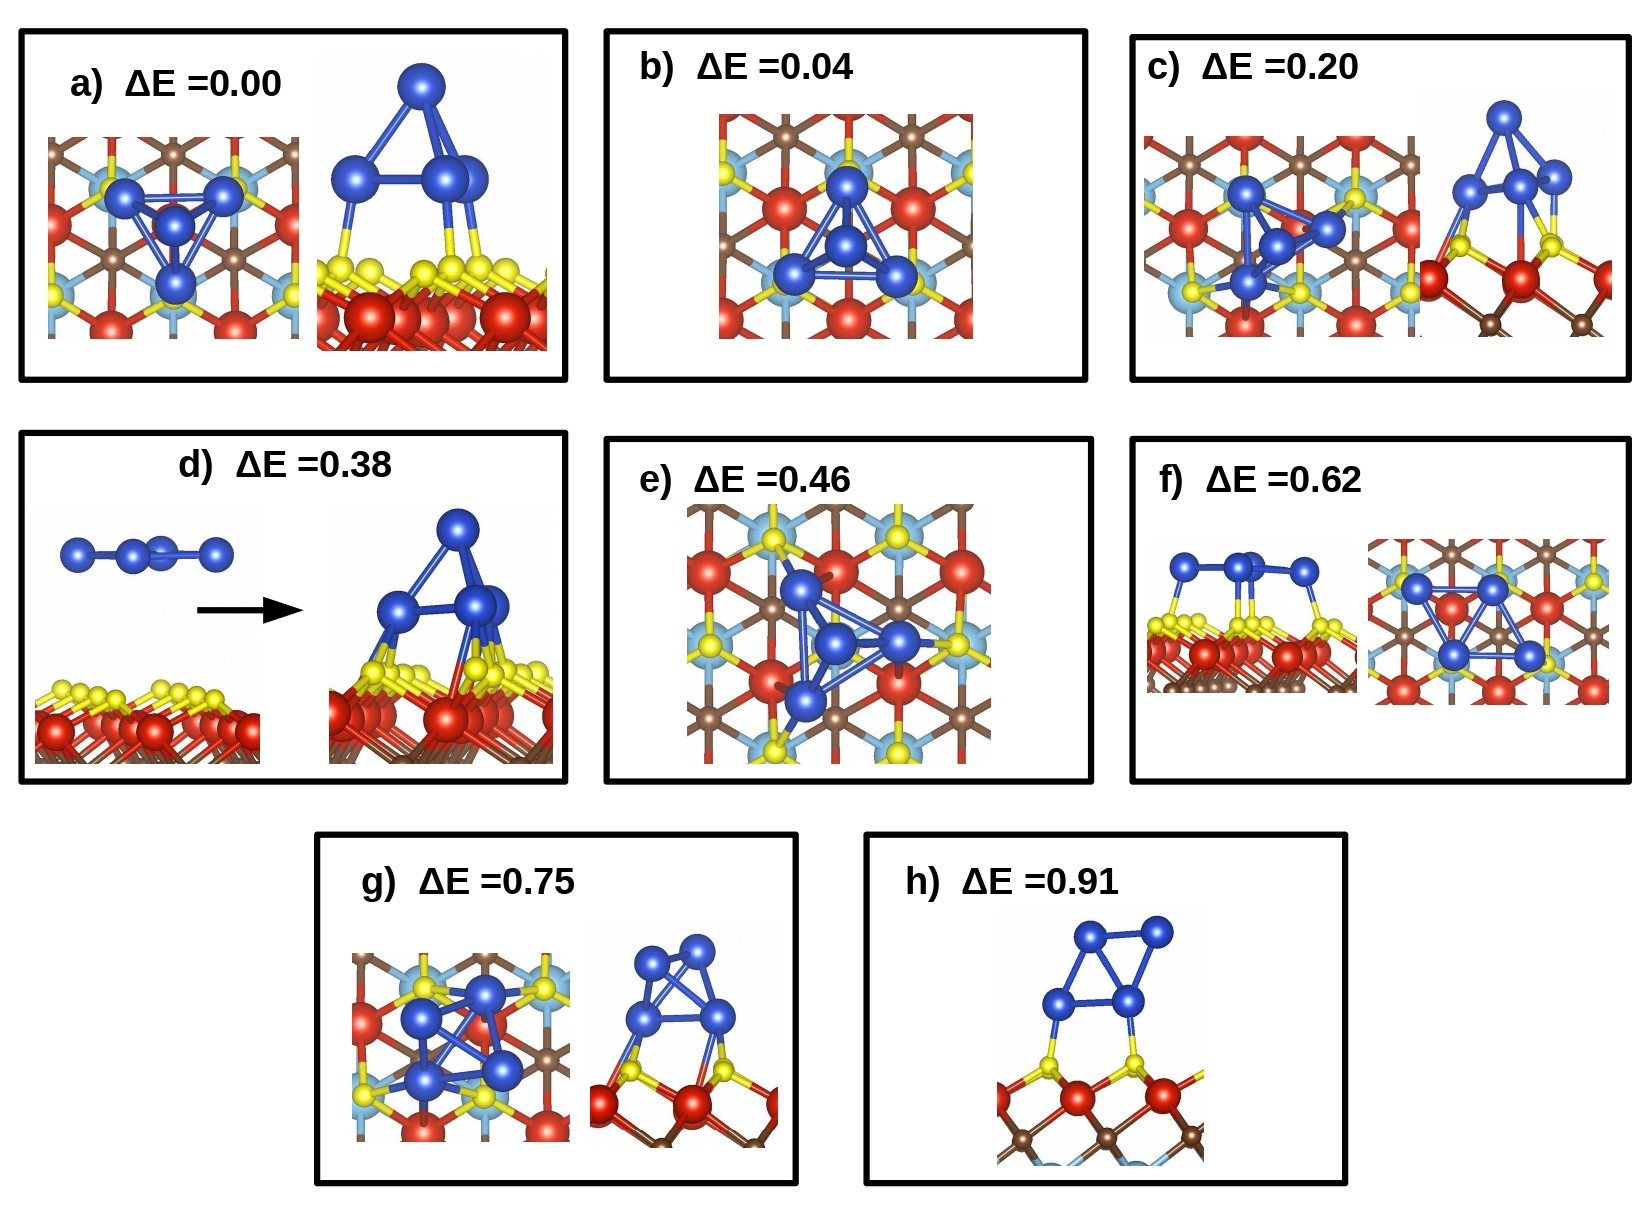
\includegraphics[width=0.9\textwidth]{./Appendix2/Appendix2_figures/photo12.jpg}
  \end{center}
    \caption{Possible tetramer configurations on O-$t$ MXene (Cu$_4$/Ti$_2$CO$_2$). $\Delta$E is the relative energy with respect to the most stable isomer.}
  \label{fig-012}
\end{figure}

\begin{figure}[htb]
  \begin{center}
    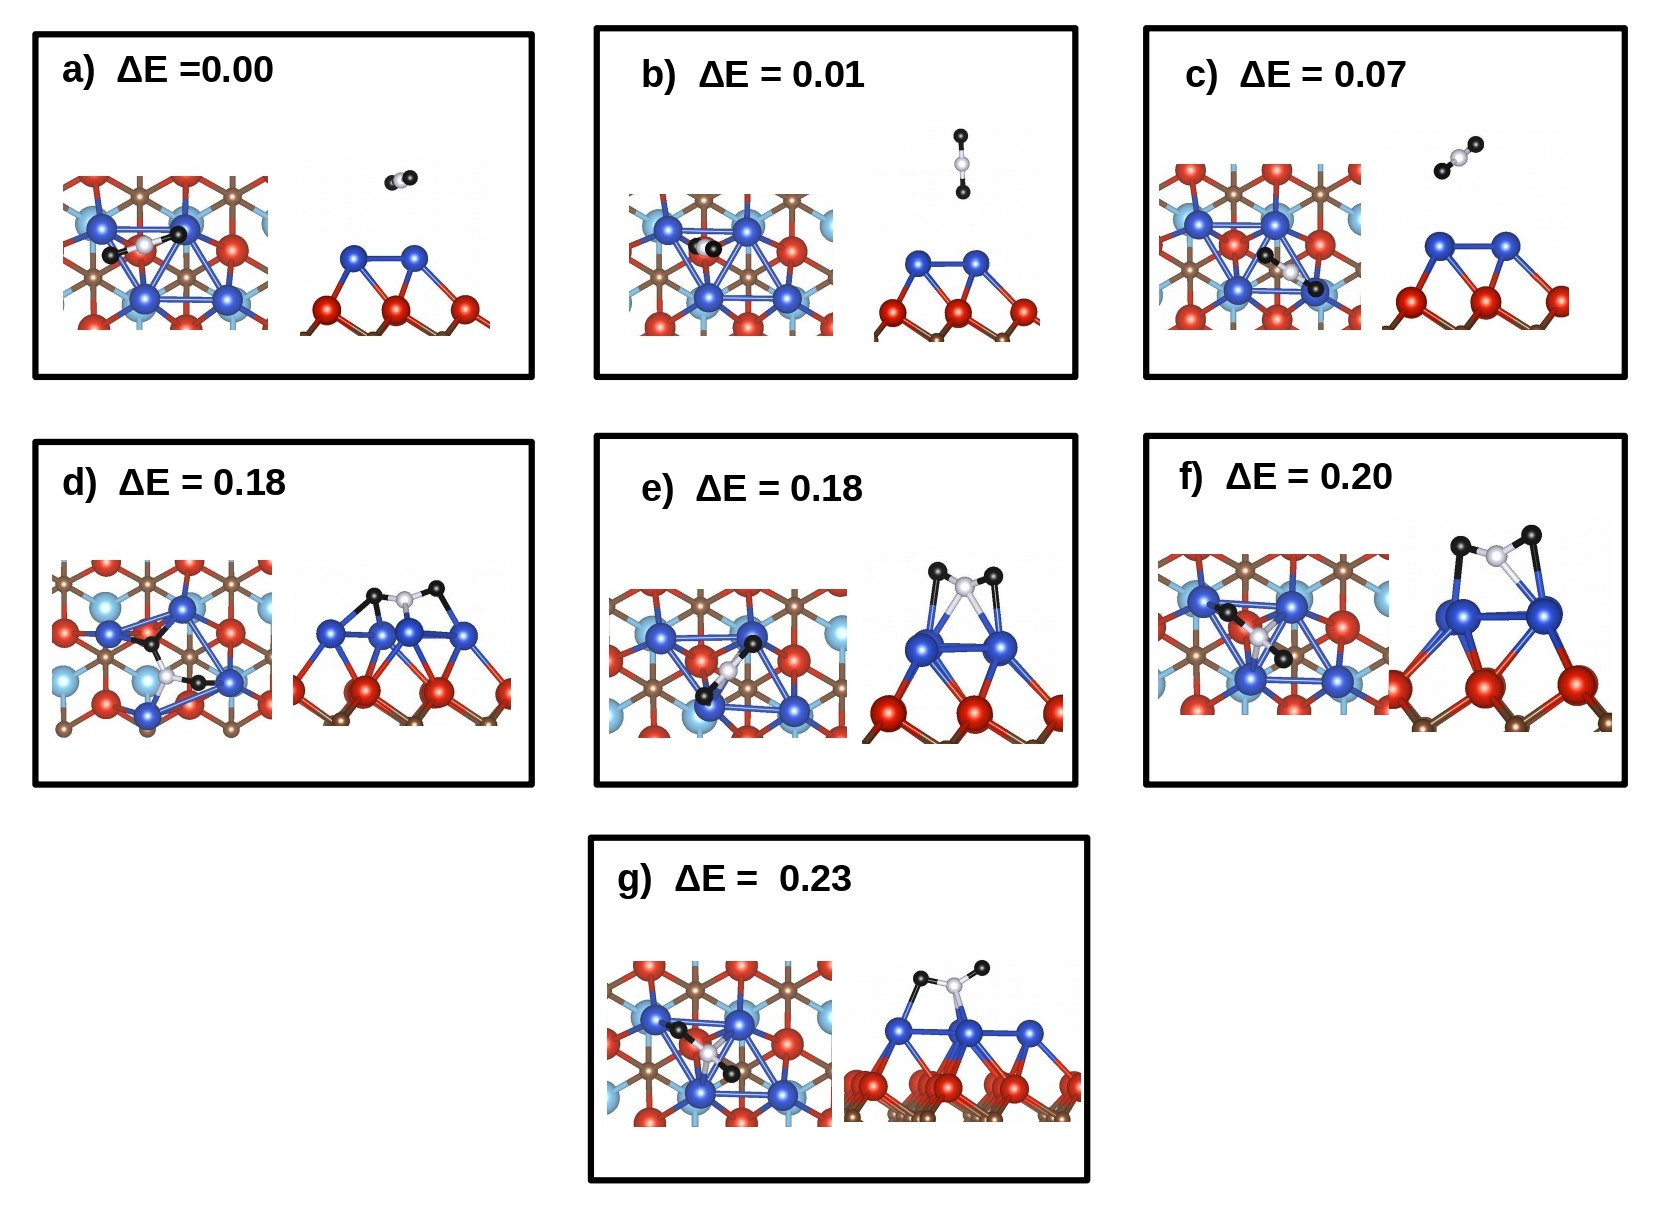
\includegraphics[width=0.9\textwidth]{./Appendix2/Appendix2_figures/photo13.jpg}
  \end{center}
    \caption{Possible CO$_2$ geometries on rhombus tetramer on pristine MXene (CO$_2$-Cu$_4$(2D)/Ti$_2$C. $\Delta$E is the relative energy with respect to the most stable isomer.}
  \label{fig-013}
\end{figure}



\begin{figure}[htb]
  \begin{center}
    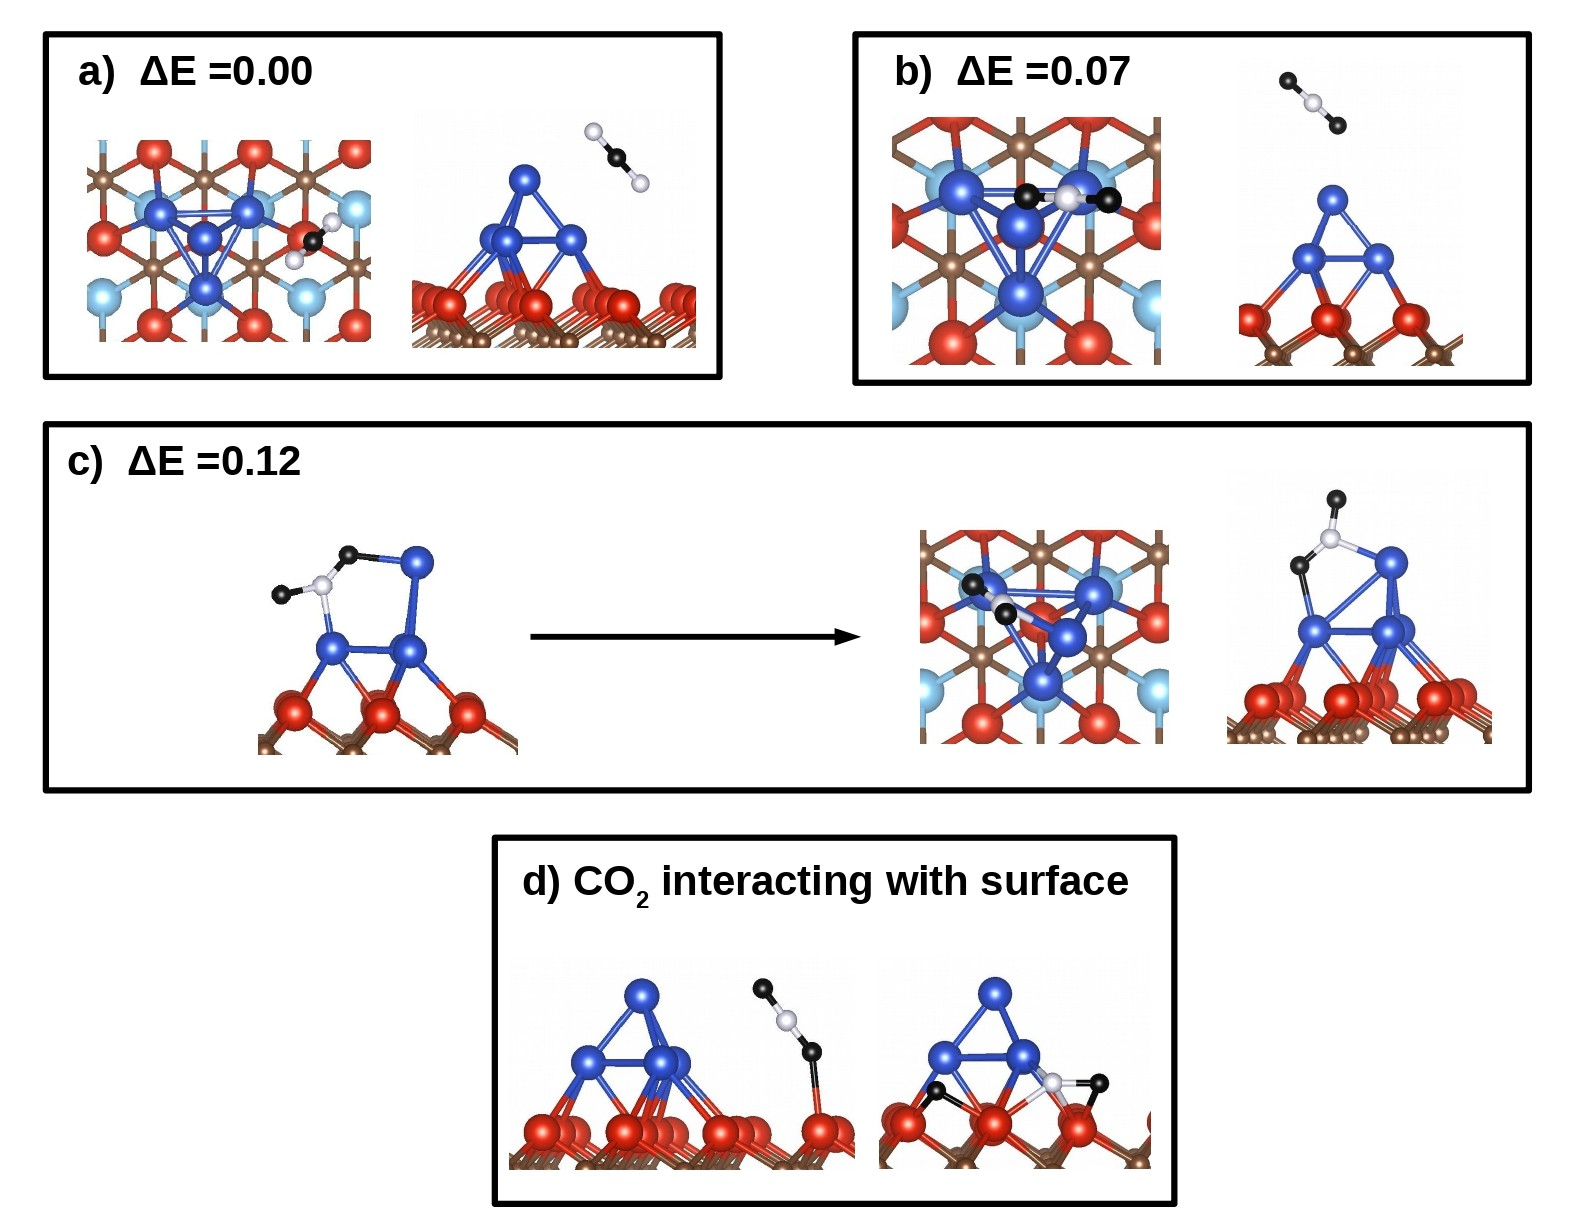
\includegraphics[width=0.9\textwidth]{./Appendix2/Appendix2_figures/photo14.jpg}
  \end{center}
\caption{Possible CO$_2$ configurations on tetrahedral tetramer on pristine MXene (CO$_2$-Cu$_4$(3D)/Ti$_2$C. $\Delta$E is the relative energy with respect to the most stable isomer.}
  \label{fig-014}
\end{figure}

\begin{figure}[htb]
  \begin{center}
    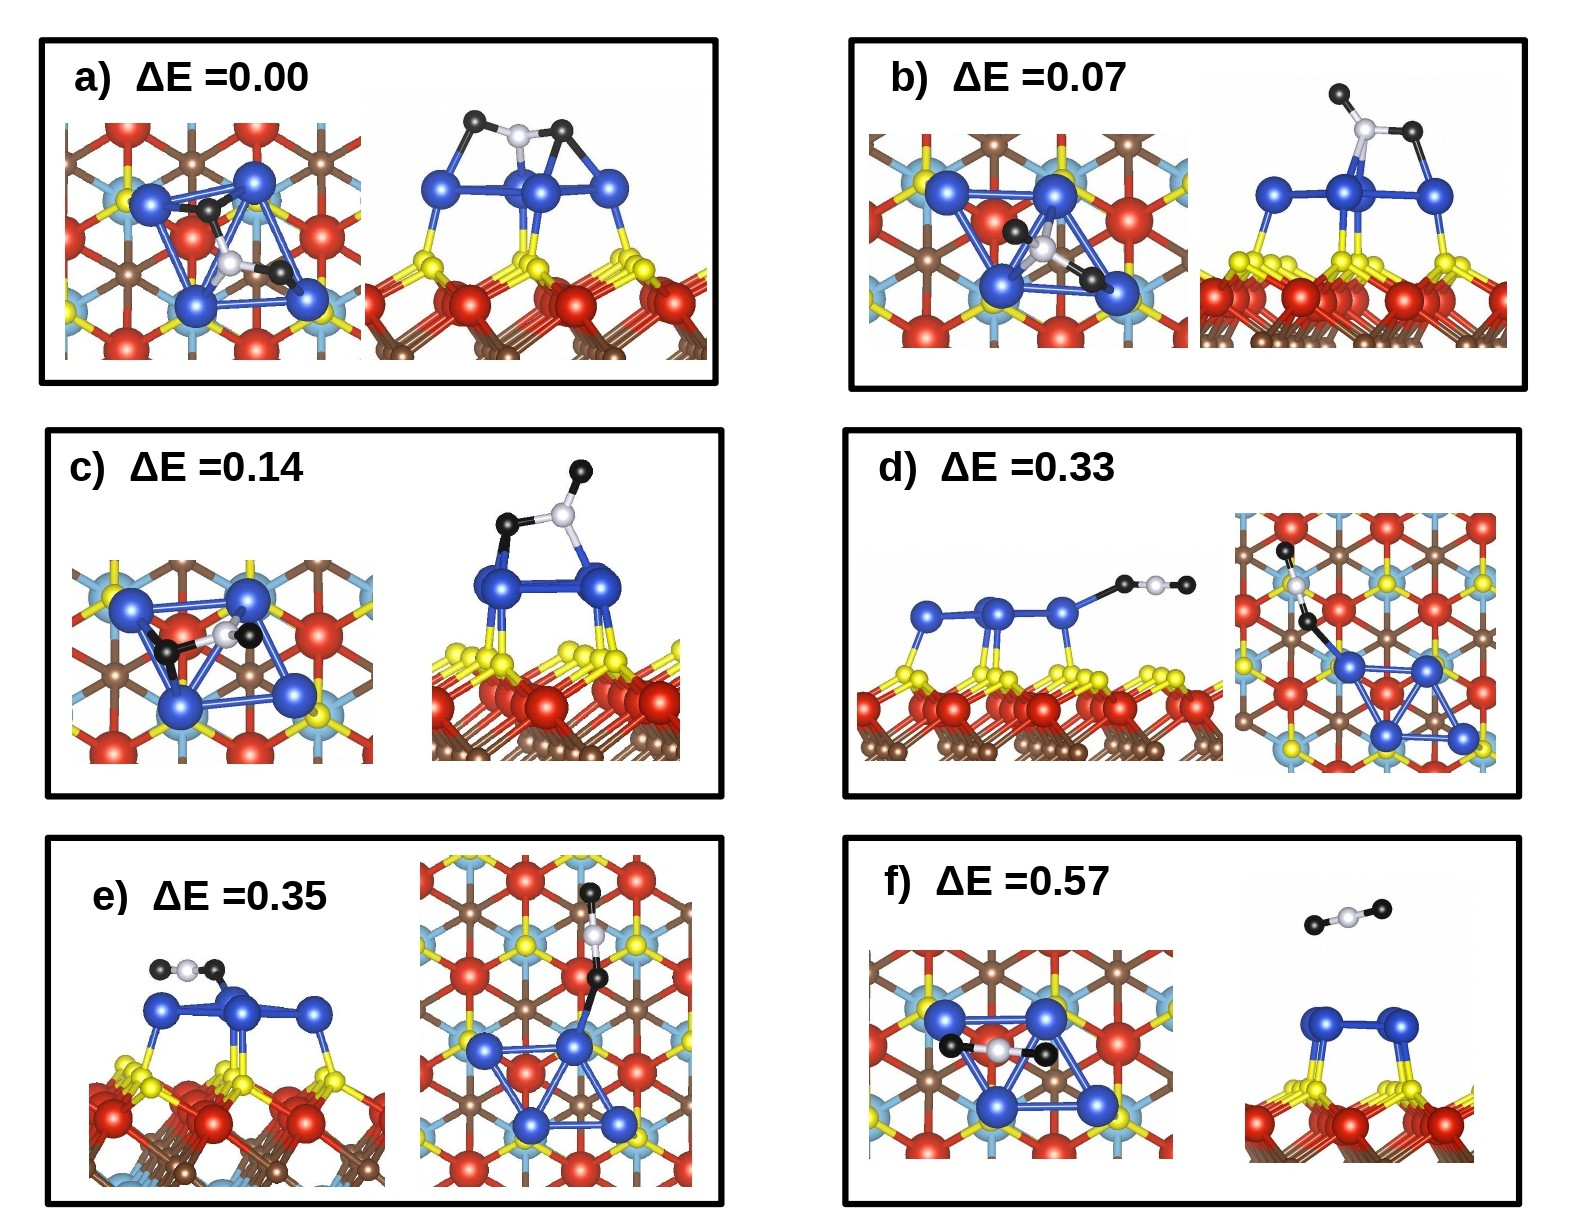
\includegraphics[width=0.9\textwidth]{./Appendix2/Appendix2_figures/photo16.jpg}
  \end{center}
\caption{Possible CO$_2$ configurations on rhombus tetramer on O-$t$ MXene (CO$_2$-Cu$_4$(2D)/Ti$_2$CO$_2$). $\Delta$E is the relative energy with respect to the most stable isomer.}
  \label{fig-016}
\end{figure}


\begin{figure}[htb]
  \begin{center}
    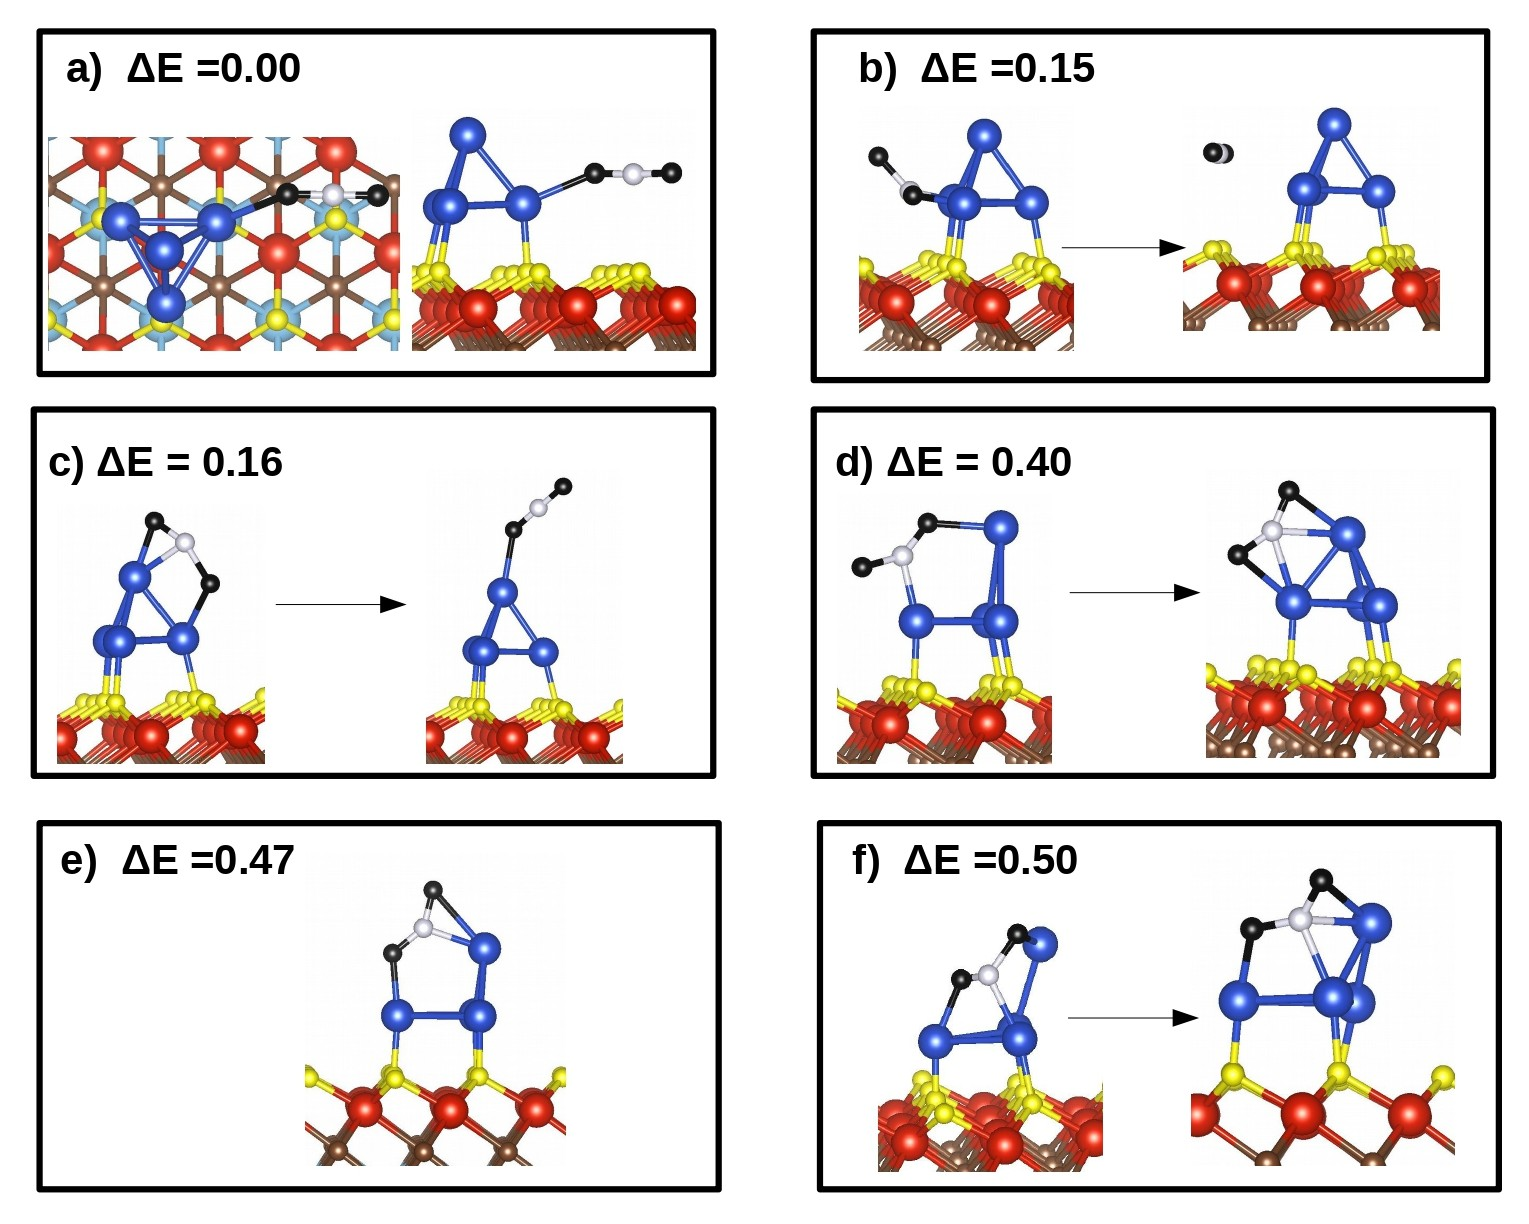
\includegraphics[width=0.9\textwidth]{./Appendix2/Appendix2_figures/photo15.jpg}
  \end{center}
   \caption{Possible CO$_2$ configurations on tetrahedral tetramer on O-$t$ MXene (CO$_2$-Cu$_4$(3D)/Ti$_2$CO$_2$). $\Delta$E is the relative energy with respect to the most stable isomer.}
  \label{fig-015}
\end{figure}

%\bibliography{appendix2.bib}
